\documentclass{beamer}

\mode<presentation>{
\usetheme{Madrid}
%\usecolortheme{beaver}
}
\usepackage[utf8]{inputenc}
%\usepackage{default}
%\usepackage[portuguese]{babel}
%\usepackage{pgfplots}
%\pgfplotsset{/pgf/number format/use comma,compat=newest}
%\usepackage{color}
\usepackage{amsfonts}
\usepackage{mathrsfs}  

%\usepackage{hyperref}


%MEUS COMANDOs

\usepackage{tikz}
\usetikzlibrary{quotes, angles, intersections}
\newcommand{\R}{\mathbb{R}}
\newcommand{\D}{\mathscr{D}}
\newcommand{\Pp}{\mathscr{P}}
\newcommand{\Cc}{\mathscr{C}}
\newcommand{\E}{\mathscr{E}}

\newcommand{\bigO}{\mathscr{O}}
\usetikzlibrary{matrix}
\usepackage{pgfplots}
\pgfplotsset{compat=1.4}
\usepackage{algorithm2e}
\usepackage{algorithmic}
\usepackage{float}
\usepackage{caption}
\newcommand{\source}[1]{\caption*{Source: {#1}} }

%\usepgfplotslibrary{external}
%\tikzexternalize
%\usepackage{natbib}

\usepackage[
backend=biber,
style=authoryear,
autocite=inline
]{biblatex}
%\DeclareLanguageMapping{english}{english-apa}

\addbibresource{../references.bib} %Imports bibliography file
%\DeclareLanguageMapping{american}{american-apa}



%FIM MEUS COMANDOS

\title[Qualificação de Mestrado]{Planar Maximal Covering with Ellipses}
\author[Tedeschi, D. F.]{Danilo F. Tedeschi\\ \small Orientadora: Dra. Marina Andretta}

\institute[ICMC]{Instituto de Ciências Matemáticas e Computação}
\date{\today}

\begin{document}

\begin{frame}
 \maketitle
 
 
\centering Agradecimentos à CAPES.
\end{frame}

\begin{frame}
\frametitle{Contents}
 \tableofcontents
\end{frame}

\section{Introduction}
\begin{frame}
\frametitle{Introduction}
\begin{itemize}
	\item Covering problems
	\begin{itemize}
		\item Minimum Cover Problem \autocite{karp}
		\item Maximal Covering Problem \autocite{church:1974}
	\end{itemize}

\end{itemize}

\begin{figure}
	\caption{Minimum Vertex Cover and its maximal counterpart. The colored edges are in the cover.}
	

\tikzset{every picture/.style={line width=0.75pt}} %set default line width to 0.75pt        

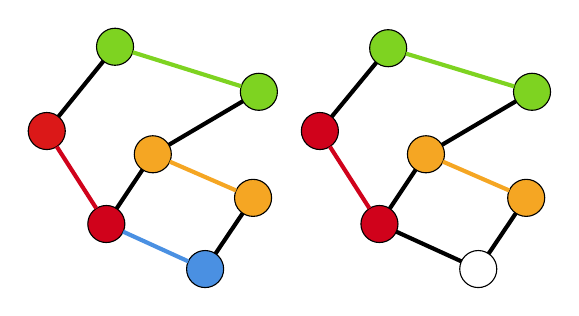
\begin{tikzpicture}[x=0.75pt,y=0.75pt,yscale=-0.7,xscale=0.7]
%uncomment if require: \path (0,300); %set diagram left start at 0, and has height of 300


% Text Node
\draw  [fill={rgb, 255:red, 126; green, 211; blue, 33 }  ,fill opacity=1 ]  (93, 74) circle [x radius= 12.75, y radius= 12.75]   ;
\draw (93,74) node [scale=0.8]  {$$};
% Text Node
\draw  [fill={rgb, 255:red, 219; green, 24; blue, 24 }  ,fill opacity=1 ]  (46, 132) circle [x radius= 12.75, y radius= 12.75]   ;
\draw (46,132) node [scale=0.8]  {$$};
% Text Node
\draw  [fill={rgb, 255:red, 126; green, 211; blue, 33 }  ,fill opacity=1 ]  (192, 105) circle [x radius= 12.75, y radius= 12.75]   ;
\draw (192,105) node [scale=0.8]  {$$};
% Text Node
\draw  [fill={rgb, 255:red, 245; green, 166; blue, 35 }  ,fill opacity=1 ]  (119, 148) circle [x radius= 12.75, y radius= 12.75]   ;
\draw (119,148) node [scale=0.8]  {$$};
% Text Node
\draw  [fill={rgb, 255:red, 245; green, 166; blue, 35 }  ,fill opacity=1 ]  (188, 178) circle [x radius= 12.75, y radius= 12.75]   ;
\draw (188,178) node [scale=0.8]  {$$};
% Text Node
\draw  [fill={rgb, 255:red, 208; green, 2; blue, 27 }  ,fill opacity=1 ]  (87, 196) circle [x radius= 12.75, y radius= 12.75]   ;
\draw (87,196) node [scale=0.8]  {$$};
% Text Node
\draw  [fill={rgb, 255:red, 74; green, 144; blue, 226 }  ,fill opacity=1 ]  (155, 227) circle [x radius= 12.75, y radius= 12.75]   ;
\draw (155,227) node [scale=0.8]  {$$};
% Text Node
\draw  [fill={rgb, 255:red, 126; green, 211; blue, 33 }  ,fill opacity=1 ]  (281, 75) circle [x radius= 12.75, y radius= 12.75]   ;
\draw (281,75) node [scale=0.8]  {$$};
% Text Node
\draw  [fill={rgb, 255:red, 208; green, 2; blue, 27 }  ,fill opacity=1 ]  (234, 132) circle [x radius= 12.75, y radius= 12.75]   ;
\draw (234,132) node [scale=0.8]  {$$};
% Text Node
\draw  [fill={rgb, 255:red, 126; green, 211; blue, 33 }  ,fill opacity=1 ]  (380, 105) circle [x radius= 12.75, y radius= 12.75]   ;
\draw (380,105) node [scale=0.8]  {$$};
% Text Node
\draw  [fill={rgb, 255:red, 245; green, 166; blue, 35 }  ,fill opacity=1 ]  (307, 148) circle [x radius= 12.75, y radius= 12.75]   ;
\draw (307,148) node [scale=0.8]  {$$};
% Text Node
\draw  [fill={rgb, 255:red, 245; green, 166; blue, 35 }  ,fill opacity=1 ]  (376, 178) circle [x radius= 12.75, y radius= 12.75]   ;
\draw (376,178) node [scale=0.8]  {$$};
% Text Node
\draw  [fill={rgb, 255:red, 208; green, 2; blue, 27 }  ,fill opacity=1 ]  (275, 196) circle [x radius= 12.75, y radius= 12.75]   ;
\draw (275,196) node [scale=0.8]  {$$};
% Text Node
\draw  [fill={rgb, 255:red, 255; green, 255; blue, 255 }  ,fill opacity=1 ]  (343, 227) circle [x radius= 12.75, y radius= 12.75]   ;
\draw (343,227) node [scale=0.8]  {$$};
% Connection
\draw [color={rgb, 255:red, 0; green, 0; blue, 0 }  ,draw opacity=1 ][line width=1.5]    (54.03,122.1) -- (84.97,83.9) ;


% Connection
\draw [color={rgb, 255:red, 126; green, 211; blue, 33 }  ,draw opacity=1 ][line width=1.5]    (179.83,101.19) -- (105.17,77.81) ;


% Connection
\draw [color={rgb, 255:red, 0; green, 0; blue, 0 }  ,draw opacity=1 ][line width=1.5]    (129.99,141.53) -- (181.01,111.47) ;


% Connection
\draw [color={rgb, 255:red, 208; green, 2; blue, 27 }  ,draw opacity=1 ][line width=1.5]    (80.12,185.26) -- (52.88,142.74) ;


% Connection
\draw [color={rgb, 255:red, 74; green, 144; blue, 226 }  ,draw opacity=1 ][line width=1.5]    (98.6,201.29) -- (143.4,221.71) ;


% Connection
\draw [color={rgb, 255:red, 0; green, 0; blue, 0 }  ,draw opacity=1 ][line width=1.5]    (162.12,216.43) -- (180.88,188.57) ;


% Connection
\draw [color={rgb, 255:red, 0; green, 0; blue, 0 }  ,draw opacity=1 ][line width=1.5]    (94.07,185.39) -- (111.93,158.61) ;


% Connection
\draw [color={rgb, 255:red, 245; green, 166; blue, 35 }  ,draw opacity=1 ][line width=1.5]    (176.31,172.92) -- (130.69,153.08) ;


% Connection
\draw [color={rgb, 255:red, 0; green, 0; blue, 0 }  ,draw opacity=1 ][line width=1.5]    (242.11,122.16) -- (272.89,84.84) ;


% Connection
\draw [color={rgb, 255:red, 126; green, 211; blue, 33 }  ,draw opacity=1 ][line width=1.5]    (367.8,101.3) -- (293.2,78.7) ;


% Connection
\draw [color={rgb, 255:red, 0; green, 0; blue, 0 }  ,draw opacity=1 ][line width=1.5]    (317.99,141.53) -- (369.01,111.47) ;


% Connection
\draw [color={rgb, 255:red, 208; green, 2; blue, 27 }  ,draw opacity=1 ][line width=1.5]    (268.12,185.26) -- (240.88,142.74) ;


% Connection
\draw [color={rgb, 255:red, 0; green, 0; blue, 0 }  ,draw opacity=1 ][line width=1.5]    (286.6,201.29) -- (331.4,221.71) ;


% Connection
\draw [color={rgb, 255:red, 0; green, 0; blue, 0 }  ,draw opacity=1 ][line width=1.5]    (350.12,216.43) -- (368.88,188.57) ;


% Connection
\draw [color={rgb, 255:red, 0; green, 0; blue, 0 }  ,draw opacity=1 ][line width=1.5]    (282.07,185.39) -- (299.93,158.61) ;


% Connection
\draw [color={rgb, 255:red, 245; green, 166; blue, 35 }  ,draw opacity=1 ][line width=1.5]    (364.31,172.92) -- (318.69,153.08) ;



\end{tikzpicture}
	
	\source{Elaborated by the author.}
\end{figure}
\end{frame}



\begin{frame}{Introduction}
\begin{itemize}

	\item Maximal Covering Location Problem (MCLP)
	
	\begin{itemize}
		\item Introduce at first for networks \autocite{church:1974}. Facilities are placed on nodes, covering a radius of neighboring vertexes.
	\end{itemize}
	\item Planar Maximal Covering Location Problem (PMCLP)
	\begin{itemize}
		\item Introduced by \autocite{church:1984}.
		\item One disk is 3SUM-Hard \autocite{3SUM-kopelowitz:2014}.
		\item One disk: $\bigO(n^2)$ and $\bigO(n^2\log{n})$ algorithms.
		\item $m$ disks: $\bigO(n^{2m-1}\log{n})$ algorithm.
	\end{itemize}
	\item Goals
	\begin{itemize}
		\item Develop a $\bigO(n^2\log{n})$ algorithm for the one disk case.
		\item Adapt it for the $m$ ellipses case creating a $\bigO(n^{2m})$ algorithm.
	\end{itemize}
\end{itemize}

\end{frame} 




%\section{Preliminaries}

%\begin{frame}{Preliminaries}
	
%	\begin{block}{Norms}
%		Let $u \in \R^2$ and $Q$ a $2x2$ positive definite matrix
%		\begin{itemize}
%			\item Euclidean
%			\begin{equation*}
%			||u||_2 = \sqrt{u^Tu}
%			\end{equation*}
%			
%			\item Elliptical
%			\begin{equation*}
%			||u||_{Q} = \sqrt{u^TQu}
%			\end{equation*}
%		\end{itemize}
%	\end{block}

%\end{frame}





\section{Maximal Covering by Disks}
\begin{frame}{Maximal Covering by Disks}{One disk}
	
	$MCD(\Pp, 1)$ is the problem of placing one disk on the plane to cover a subset of a demand set $\Pp$, with $n$ points, maximizing the weights of the covered points.
	
	\begin{equation*}\label{eq:max_one_disk}
		\max_q w(\Pp \cap D(q)),
	\end{equation*}
	
	\begin{itemize}
		\item $\Pp=\{p_1,\dots,p_n\}$ is the demand set with weights $w(p_i)>0$.
		\item $w(A)$, $A\subset \Pp$, is the sum of weights of the points in $A$.
		\item $D(q)$ is a unit disk with center at point $q$.
		%\item \autocite{chazelle:1986} proposed a $\bigO(n^2)$ algorithm
		%\item \autocite{drezner} proposed a $\bigO(n^2\log{n})$ which our work is based on
		%\item We will introduce an equivalent problem...
	\end{itemize}
\end{frame}

\begin{frame}{Maximal Covering by Disks}{One disk}
\begin{figure}
	\caption{An instance of $MCD(\Pp,1)$.}
	\includegraphics[scale=0.6]{figures/mcd_one_disk.pdf}
	\source{Elaborated by the author.}
\end{figure}
\end{frame}

\begin{frame}{Maximal Covering By Disks}{One disk}
	
	Works and results found in the literature:
	
	\begin{itemize}
		\item $MCD$ is as difficult the problem of given $n$ numbers, find three of them that sum to $0$ (3SUM-HARD). Proved by \autocite{aronov:2008}.
		
		\item In \autocite{drezner} a $\bigO(n^2\log{n})$ algorithm was developed. The idea of our algorithm to sort the intersections by their angles comes from here.
		
		\item In \autocite{chazelle:1986}, a $\bigO(n^2)$ algorithm was developed. It actually solves an equivalent problem which is introduced next.
	\end{itemize}
	
	
	
\end{frame}

\subsection{Maximum Weight Clique Problem}
\begin{frame}{Maximum Weight Clique Problem}
	Let $\D=\{D_1,\dots,D_n\}$ be a set of $n$ unit disks with weights $w_i>0$. The maximum weight clique is defined as
	
	\begin{equation*}
	\max_{q\in\R^2} \sum_{D_k \cap q \neq \emptyset} w_k,
	\end{equation*}
	
	\begin{itemize}
		\item A clique is a non-empty intersection area of a subset of disks. We search for only a point in an optimal clique.
		
		\item The weight of a clique is the sum of the weights of the disks that intersect with it.
		
		\item In our case, we just want a point from the optimum clique.
		
		\item Given an instance $MCD(\Pp, 1)$: fix the disk centers at $\Pp =\{p_1,\dots,p_n\}$ with weights $w_k=w(p_k)$.

		%\item An optimal solution for the maximum weight clique is an optimal solution for $MCD(\Pp,1)$.
	\end{itemize}
\end{frame}

\begin{frame}{Maximum Weight Clique Problem}{Equivalence}
	\begin{figure}
		\only<1>{\caption{An instance of $MCD(\Pp, 1)$. We will show how an instance of the Maximum Weight Clique Problem is constructed from it.}}
		\only<2>{\caption{An instance of the Maximum Weight Clique Problem obtained from an instance of $MCD(\Pp, 1)$.}}
		\only<3>{\caption{An instance of the Maximum Weight Clique Problem obtained from an instance of $MCD(\Pp, 1)$. In gray, the optimal solution.}}
		\only<1>{\includegraphics[scale=0.50]{figures/mwc_1.pdf}}
		\only<2>{\includegraphics[scale=0.50]{figures/mwc_2.pdf}}
		\only<3>{\includegraphics[scale=0.50]{figures/mwc_3.pdf}}
		%\only<2>{\input{figures/intro_b.tex}}
		\source{Elaborated by the author.}
	\end{figure}
\end{frame}

%\begin{frame}{Maximum Weight Clique Problem}{Equivalence}
%		\begin{figure}[H]
%		\centering
		
%		\only<1>{}
		
%		\only<2>{\caption{An instance of the Maximum Weight Clique Problem obtained from an instance of $MCD(\Pp, 1)$. In gray, the optimal solution.}}
		
%		\only<1>{% This file was created by matplotlib2tikz v0.7.4.
\begin{tikzpicture}

\begin{axis}[
tick align=outside,
tick pos=left,
x grid style={white!69.01960784313725!black},
xmin=-2, xmax=2,
xtick style={color=black},
y grid style={white!69.01960784313725!black},
ymin=-2, ymax=2,
ytick style={color=black}
]
\addplot [only marks, draw=red, fill=red, colormap/viridis]
table{%
	x                      y
	-0.8 -0.2
	-0.2 0.4
	0.9 -0.4
};
\path [draw=black, fill=red, opacity=0.2]
(axis cs:0.2,-0.2)
--(axis cs:0.195184726672197,-0.298017140329561)
--(axis cs:0.18078528040323,-0.395090322016128)
--(axis cs:0.156940335732209,-0.490284677254462)
--(axis cs:0.139375395780243,-0.539375395780243)
--(axis cs:0.0902846772544636,-0.556940335732208)
--(axis cs:-0.00490967798387038,-0.58078528040323)
--(axis cs:-0.0812279586139392,-0.59210602792772)
--(axis cs:-0.0951847266721968,-0.498017140329562)
--(axis cs:-0.1,-0.400000000000001)
--(axis cs:-0.0951847266721969,-0.30198285967044)
--(axis cs:-0.0807852804032306,-0.204909677983873)
--(axis cs:-0.056940335732209,-0.109715322745538)
--(axis cs:-0.0238795325112869,-0.0173165676349108)
--(axis cs:0.0180787356516448,0.0713967368259972)
--(axis cs:0.0685303876974546,0.155570233019602)
--(axis cs:0.110157019435624,0.211697248562716)
--(axis cs:0.123879532511284,0.182683432365096)
--(axis cs:0.156940335732207,0.0902846772544693)
--(axis cs:0.180785280403229,-0.00490967798386432)
--(axis cs:0.195184726672196,-0.101982859670432)
--(axis cs:0.2,-0.199999999999992)
--(axis cs:0.2,-0.2);
\draw (-0.8,-0.2) circle (1);
\draw (axis cs:-0.2,0.4) circle (1);
\draw(axis cs:0.9,-0.4) circle (1);
\end{axis}

\end{tikzpicture}}
%		\only<2>{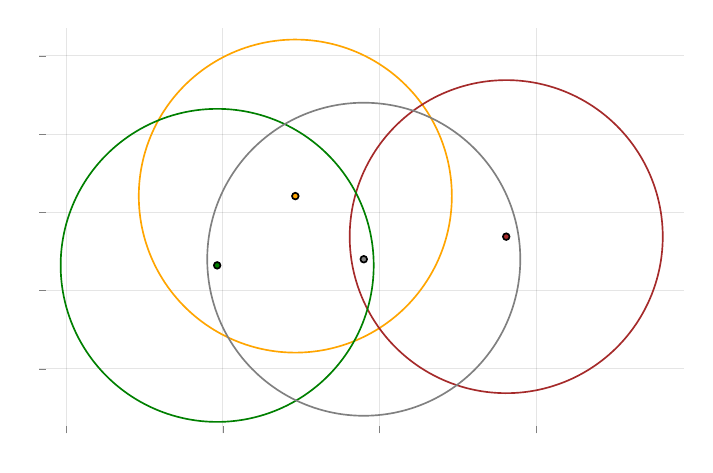
\begin{tikzpicture}[scale=0.6]
\begin{axis}[height = {101.6mm}, axis equal = {true}, ylabel = {}, xmin = {-0.15165998854733476}, xmax = {3.925522135163323}, ymax = {2.176713972397551}, xlabel = {}, unbounded coords=jump,scaled x ticks = false,xlabel style = {font = {\fontsize{11 pt}{14.3 pt}\selectfont}, color = {rgb,1:red,0.00000000;green,0.00000000;blue,0.00000000}, draw opacity = 1.0, rotate = 0.0},xmajorgrids = true,xtick = {0.0,1.0,2.0,3.0},xticklabels = {},xtick align = inside,xticklabel style = {font = {\fontsize{8 pt}{10.4 pt}\selectfont}, color = {rgb,1:red,0.00000000;green,0.00000000;blue,0.00000000}, draw opacity = 1.0, rotate = 0.0},x grid style = {color = {rgb,1:red,0.00000000;green,0.00000000;blue,0.00000000},
draw opacity = 0.1,
line width = 0.5,
solid},axis lines* = left,separate axis lines,x axis line style = {draw opacity = 0},scaled y ticks = false,ylabel style = {font = {\fontsize{11 pt}{14.3 pt}\selectfont}, color = {rgb,1:red,0.00000000;green,0.00000000;blue,0.00000000}, draw opacity = 1.0, rotate = 0.0},ymajorgrids = true,ytick = {0.0,0.5,1.0,1.5,2.0},yticklabels = {},ytick align = inside,yticklabel style = {font = {\fontsize{8 pt}{10.4 pt}\selectfont}, color = {rgb,1:red,0.00000000;green,0.00000000;blue,0.00000000}, draw opacity = 1.0, rotate = 0.0},y grid style = {color = {rgb,1:red,0.00000000;green,0.00000000;blue,0.00000000},
draw opacity = 0.1,
line width = 0.5,
solid},axis lines* = left,separate axis lines,y axis line style = {draw opacity = 0},    xshift = 0.0mm,
    yshift = 0.0mm,
    axis background/.style={fill={rgb,1:red,1.00000000;green,1.00000000;blue,1.00000000}}
,legend style = {color = {rgb,1:red,0.00000000;green,0.00000000;blue,0.00000000},
draw opacity = 1.0,
line width = 1,
solid,fill = {rgb,1:red,1.00000000;green,1.00000000;blue,1.00000000},font = {\fontsize{8 pt}{10.4 pt}\selectfont}},colorbar style={title=}, ymin = {-0.4124307900072879}, width = {152.4mm}]\addplot+[draw=none, color = {rgb,1:red,1.00000000;green,0.64705882;blue,0.00000000},
draw opacity = 1.0,
line width = 0,
solid,mark = *,
mark size = 2.0,
mark options = {
    color = {rgb,1:red,0.00000000;green,0.00000000;blue,0.00000000}, draw opacity = 1.0,
    fill = {rgb,1:red,1.00000000;green,0.64705882;blue,0.00000000}, fill opacity = 1.0,
    line width = 1,
    rotate = 0,
    solid
},forget plot] coordinates {
(1.4627452129931668, 1.1034674435485403)
};
\addplot+[draw=none, color = {rgb,1:red,0.64705882;green,0.16470588;blue,0.16470588},
draw opacity = 1.0,
line width = 0,
solid,mark = *,
mark size = 2.0,
mark options = {
    color = {rgb,1:red,0.00000000;green,0.00000000;blue,0.00000000}, draw opacity = 1.0,
    fill = {rgb,1:red,0.64705882;green,0.16470588;blue,0.16470588}, fill opacity = 1.0,
    line width = 1,
    rotate = 0,
    solid
},forget plot] coordinates {
(2.810130188265852, 0.844338567963324)
};
\addplot+[draw=none, color = {rgb,1:red,0.00000000;green,0.50196078;blue,0.00000000},
draw opacity = 1.0,
line width = 0,
solid,mark = *,
mark size = 2.0,
mark options = {
    color = {rgb,1:red,0.00000000;green,0.00000000;blue,0.00000000}, draw opacity = 1.0,
    fill = {rgb,1:red,0.00000000;green,0.50196078;blue,0.00000000}, fill opacity = 1.0,
    line width = 1,
    rotate = 0,
    solid
},forget plot] coordinates {
(0.963607347867794, 0.6608157388417224)
};
\addplot+ [color = {rgb,1:red,1.00000000;green,0.64705882;blue,0.00000000},
draw opacity = 1.0,
line width = 1,
solid,mark = none,
mark size = 2.0,
mark options = {
    color = {rgb,1:red,0.00000000;green,0.00000000;blue,0.00000000}, draw opacity = 1.0,
    fill = {rgb,1:red,1.00000000;green,0.64705882;blue,0.00000000}, fill opacity = 1.0,
    line width = 1,
    rotate = 0,
    solid
},forget plot]coordinates {
(2.462745212993167, 1.1034674435485403)
(2.4622468021193407, 1.135035993313351)
(2.4607520663246603, 1.166573074861214)
(2.4582624955942727, 1.1980472513433853)
(2.454780571586425, 1.2294271486162578)
(2.4503097651586905, 1.2606814865157911)
(2.4448545329081472, 1.291779110038258)
(2.4384203127289403, 1.3226890203962316)
(2.431013518391674, 1.3533804059188488)
(2.4226415331500237, 1.3838226727655547)
(2.4133127023809497, 1.413985475422709)
(2.4030363252658424, 1.443838746952653)
(2.3918226455208975, 1.4733527289650872)
(2.3796828411859554, 1.5024980012808813)
(2.3666290134819903, 1.53124551125875)
(2.3526741747483473, 1.5595666027555564)
(2.3378322354717604, 1.5874330446913791)
(2.322117990420079, 1.614817059190867)
(2.3055471038945177, 1.6416913492728287)
(2.288136094115143, 1.6680291260604583)
(2.269902316755152, 1.6938041354850686)
(2.2508639476403594, 1.7189906844567195)
(2.2310399646311376, 1.7435636664756475)
(2.210450128704876, 1.7674985866589714)
(2.189114964257806, 1.7907715861577245)
(2.167055738645839, 1.813359465939873)
(2.1442944409848006, 1.835239709915617)
(2.1208537602312045, 1.8563905073819174)
(2.0967570625654055, 1.8767907747638795)
(2.0720283680996836, 1.896420176631319)
(2.046692326934473, 1.9152591459695611)
(2.020774194586607, 1.9332889036842662)
(1.9942998068140683, 1.9504914773208393)
(1.9672955538623444, 1.9668497189797636)
(1.9397883541580563, 1.9823473224100008)
(1.911805627476087, 1.9969688392634144)
(1.8833752676069513, 2.0106996944940216)
(1.85452561455166, 2.0235262008867148)
(1.8252854262717912, 2.035435572700975)
(1.795683850022928, 2.0464159384159775)
(1.7657503933000396, 2.0564563525643793)
(1.73551489442377, 2.0655468066430034)
(1.70500749279695, 2.0736782390895265)
(1.674258598860986, 2.0808425443152476)
(1.6432988637820691, 2.08703258078491)
(1.6121591488974278, 2.092242178135543)
(1.5808704949520749, 2.09646614332721)
(1.5494640911567177, 2.099700265819547)
(1.517971244097675, 2.101941321768919)
(1.486423346529791, 2.1031870772420183)
(1.4548518460834536, 2.103436290442697)
(1.423288213916914, 2.102688712949816)
(1.3917639133451511, 2.1009450899648794)
(1.3603103684765536, 2.0982071595691973)
(1.3289589328886877, 2.0944776509913323)
(1.2977408583743677, 2.089760281886543)
(1.2666872637891888, 2.0840597546309443)
(1.2358291040315768, 2.077381751634078)
(1.2051971391862701, 2.0697329296745623)
(1.1748219038620005, 2.06112091326447)
(1.1447336767539287, 2.0515542870490497)
(1.1149624504611846, 2.0410425872493656)
(1.085537901589591, 2.0295962921563815)
(1.056489361169378, 2.017226811685977)
(1.027845785417374, 2.003946476005292)
(0.9996357268728191, 1.989768523241749)
(0.9718873059355733, 1.974707086287)
(0.9446281828350896, 1.9587771787089523)
(0.9178855300580964, 1.9419946797859176)
(0.8916860052624721, 1.924376318677803)
(0.8660557247043109, 1.9059396577501184)
(0.8410202372046718, 1.8867030750674307)
(0.8166044986819573, 1.866685746073709)
(0.7928328472753116, 1.8459076244778232)
(0.7697289790838351, 1.8243894223632566)
(0.7473159245457957, 1.8021525895418469)
(0.725616025481388, 1.779219292172149)
(0.7046509128219215, 1.755612390663727)
(0.6844414850476368, 1.7313554168893988)
(0.6650078873556475, 1.7064725507281548)
(0.6463694915787678, 1.680988595962129)
(0.6285448768752494, 1.654928955551648)
(0.6115518112086723, 1.6283196063130088)
(0.5954072336364523, 1.6011870730242237)
(0.5801272374246199, 1.5735584019845432)
(0.5657270540057033, 1.5454611340541193)
(0.5522210377957046, 1.5169232772006744)
(0.5396226518853062, 1.4879732785805513)
(0.5279444546195686, 1.458639996181969)
(0.5171980870794998, 1.4289526700587518)
(0.5073942614779721, 1.3989408931832104)
(0.49854275048155516, 1.368634581947219)
(0.4906523774689099, 1.3380639463409092)
(0.4837310077354524, 1.3072594598386926)
(0.47778554065305645, 1.2762518290226401)
(0.4728219027926097, 1.2450719629734919)
(0.4688450420162791, 1.2137509424598154)
(0.46585892254537364, 1.182319988956017)
(0.4638665210087233, 1.1508104335200986)
(0.46286982347550953, 1.1192536855621775)
(0.46286982347550953, 1.0876812015349033)
(0.4638665210087233, 1.0561244535769823)
(0.46585892254537364, 1.0246148981410639)
(0.46884504201627897, 0.9931839446372654)
(0.4728219027926096, 0.961862924123589)
(0.47778554065305634, 0.9306830580744407)
(0.4837310077354523, 0.8996754272583882)
(0.4906523774689099, 0.8688709407561717)
(0.49854275048155505, 0.8383003051498619)
(0.507394261477972, 0.8079939939138705)
(0.5171980870794997, 0.7779822170383289)
(0.5279444546195685, 0.7482948909151119)
(0.5396226518853061, 0.7189616085165296)
(0.5522210377957046, 0.6900116098964064)
(0.5657270540057032, 0.6614737530429614)
(0.5801272374246198, 0.6333764851125376)
(0.5954072336364522, 0.6057478140728572)
(0.6115518112086722, 0.578615280784072)
(0.6285448768752493, 0.552005931545433)
(0.6463694915787677, 0.5259462911349518)
(0.6650078873556473, 0.500462336368926)
(0.6844414850476367, 0.4755794702076822)
(0.7046509128219213, 0.45132249643335376)
(0.7256160254813878, 0.4277155949249316)
(0.7473159245457954, 0.404782297555234)
(0.7697289790838349, 0.3825454647338241)
(0.7928328472753114, 0.36102726261925744)
(0.8166044986819567, 0.3402491410233721)
(0.8410202372046716, 0.3202318120296499)
(0.8660557247043104, 0.30099522934696277)
(0.8916860052624719, 0.28255856841927784)
(0.9178855300580965, 0.26494020731116286)
(0.9446281828350891, 0.24815770838812867)
(0.971887305935573, 0.23222780081008076)
(0.9996357268728185, 0.21716636385533195)
(1.0278457854173737, 0.20298841109178878)
(1.056489361169378, 0.18970807541110357)
(1.0855379015895905, 0.17733859494069926)
(1.1149624504611844, 0.16589229984771525)
(1.144733676753928, 0.155380600048031)
(1.1748219038620002, 0.14581397383261085)
(1.2051971391862704, 0.1372019574225184)
(1.2358291040315763, 0.12955313546300262)
(1.2666872637891888, 0.12287513246613624)
(1.297740858374367, 0.11717460521053769)
(1.3289589328886875, 0.1124572361057482)
(1.3603103684765538, 0.10872772752788329)
(1.3917639133451507, 0.10598979713220158)
(1.423288213916914, 0.10424617414726467)
(1.454851846083453, 0.10349859665438399)
(1.4864233465297907, 0.10374780985506238)
(1.5179712440976751, 0.10499356532816151)
(1.5494640911567172, 0.10723462127753358)
(1.5808704949520749, 0.1104687437698707)
(1.6121591488974274, 0.11469270896153771)
(1.643298863782069, 0.11990230631217036)
(1.6742585988609862, 0.12609234278183312)
(1.7050074927969499, 0.133256648007554)
(1.73551489442377, 0.14138808045407747)
(1.7657503933000391, 0.15047853453270088)
(1.795683850022928, 0.16051894868110328)
(1.8252854262717908, 0.17149931439610522)
(1.8545256145516598, 0.18340868621036577)
(1.8833752676069513, 0.196235192603059)
(1.9118056274760866, 0.20996604783366601)
(1.9397883541580563, 0.22458756468707997)
(1.9672955538623438, 0.24008516811731662)
(1.994299806814068, 0.25644340977624136)
(2.020774194586607, 0.27364598341281454)
(2.0466923269344726, 0.2916757411275194)
(2.0720283680996836, 0.31051471046576173)
(2.096757062565405, 0.33014411233320085)
(2.1208537602312045, 0.35054437971516317)
(2.144294440984801, 0.3716951771814636)
(2.1670557386458387, 0.3935754211572071)
(2.189114964257806, 0.41616330093935605)
(2.2104501287048754, 0.43943630043810866)
(2.2310399646311376, 0.463371220621433)
(2.2508639476403594, 0.4879442026403613)
(2.269902316755152, 0.5131307516120116)
(2.288136094115143, 0.5389057610366222)
(2.3055471038945172, 0.5652435378242513)
(2.322117990420079, 0.5921178279062135)
(2.337832235471761, 0.6195018424057017)
(2.352674174748347, 0.647368284341524)
(2.3666290134819903, 0.6756893758383308)
(2.3796828411859554, 0.7044368858161989)
(2.3918226455208975, 0.7335821581319933)
(2.403036325265842, 0.7630961401444268)
(2.4133127023809497, 0.7929494116743712)
(2.4226415331500237, 0.8231122143315259)
(2.4310135183916737, 0.8535544811782315)
(2.4384203127289403, 0.8842458667008488)
(2.4448545329081472, 0.9151557770588219)
(2.4503097651586905, 0.9462534005812893)
(2.454780571586425, 0.9775077384808228)
(2.4582624955942727, 1.008887635753695)
(2.4607520663246603, 1.0403618122358667)
(2.4622468021193407, 1.0718988937837293)
(2.462745212993167, 1.10346744354854)
};
\addplot+ [color = {rgb,1:red,0.64705882;green,0.16470588;blue,0.16470588},
draw opacity = 1.0,
line width = 1,
solid,mark = none,
mark size = 2.0,
mark options = {
    color = {rgb,1:red,0.00000000;green,0.00000000;blue,0.00000000}, draw opacity = 1.0,
    fill = {rgb,1:red,0.64705882;green,0.16470588;blue,0.16470588}, fill opacity = 1.0,
    line width = 1,
    rotate = 0,
    solid
},forget plot]coordinates {
(3.810130188265852, 0.844338567963324)
(3.809631777392026, 0.8759071177281345)
(3.8081370415973455, 0.9074441992759976)
(3.805647470866958, 0.9389183757581689)
(3.8021655468591096, 0.9702982730310415)
(3.7976947404313757, 1.0015526109305748)
(3.792239508180832, 1.0326502344530417)
(3.7858052880016255, 1.0635601448110152)
(3.778398493664359, 1.0942515303336324)
(3.770026508422709, 1.1246937971803384)
(3.760697677653635, 1.1548565998374927)
(3.7504213005385276, 1.1847098713674367)
(3.7392076207935823, 1.2142238533798708)
(3.7270678164586406, 1.243369125695665)
(3.7140139887546755, 1.2721166356735336)
(3.700059150021032, 1.30043772717034)
(3.6852172107444456, 1.3283041691061628)
(3.6695029656927636, 1.3556881836056507)
(3.6529320791672024, 1.3825624736876123)
(3.635521069387828, 1.408900250475242)
(3.617287292027837, 1.4346752598998522)
(3.598248922913044, 1.4598618088715032)
(3.5784249399038224, 1.4844347908904312)
(3.557835103977561, 1.508369711073755)
(3.5364999395304912, 1.5316427105725081)
(3.514440713918524, 1.5542305903546567)
(3.491679416257486, 1.5761108343304007)
(3.4682387355038893, 1.597261631796701)
(3.4441420378380903, 1.617661899178663)
(3.4194133433723684, 1.6372913010461025)
(3.394077302207158, 1.6561302703843448)
(3.368159169859292, 1.6741600280990498)
(3.3416847820867535, 1.691362601735623)
(3.314680529135029, 1.7077208433945472)
(3.2871733294307415, 1.7232184468247844)
(3.259190602748772, 1.737839963678198)
(3.230760242879636, 1.7515708189088053)
(3.2019105898243447, 1.7643973253014984)
(3.1726704015444764, 1.7763066971157588)
(3.1430688252956127, 1.787287062830761)
(3.1131353685727245, 1.7973274769791632)
(3.082899869696455, 1.8064179310577868)
(3.052392468069635, 1.8145493635043102)
(3.021643574133671, 1.8217136687300313)
(2.9906838390547543, 1.8279037051996938)
(2.9595441241701126, 1.8331133025503266)
(2.92825547022476, 1.8373372677419937)
(2.896849066429403, 1.8405713902343308)
(2.86535621937036, 1.8428124461837028)
(2.833808321802476, 1.844058201656802)
(2.8022368213561384, 1.8443074148574803)
(2.770673189189599, 1.8435598373645996)
(2.739148888617836, 1.8418162143796628)
(2.7076953437492386, 1.839078283983981)
(2.676343908161373, 1.835348775406116)
(2.645125833647053, 1.8306314063013267)
(2.6140722390618736, 1.824930879045728)
(2.5832140793042617, 1.8182528760488617)
(2.5525821144589553, 1.8106040540893458)
(2.5222068791346857, 1.8019920376792535)
(2.4921186520266136, 1.7924254114638334)
(2.4623474257338693, 1.781913711664149)
(2.4329228768622757, 1.7704674165711651)
(2.4038743364420627, 1.7580979361007607)
(2.3752307606900587, 1.7448176004200757)
(2.347020702145504, 1.7306396476565327)
(2.3192722812082582, 1.7155782107017836)
(2.2920131581077747, 1.699648303123736)
(2.2652705053307813, 1.6828658042007012)
(2.239070980535157, 1.6652474430925865)
(2.2134406999769958, 1.646810782164902)
(2.188405212477357, 1.6275741994822144)
(2.163989473954642, 1.6075568704884926)
(2.1402178225479966, 1.5867787488926068)
(2.11711395435652, 1.5652605467780403)
(2.0947008998184806, 1.5430237139566305)
(2.073001000754073, 1.5200904165869327)
(2.0520358880946064, 1.4964835150785107)
(2.031826460320322, 1.4722265413041824)
(2.0123928626283325, 1.4473436751429385)
(1.9937544668514526, 1.4218597203769126)
(1.9759298521479343, 1.3958000799664316)
(1.9589367864813574, 1.3691907307277924)
(1.9427922089091374, 1.3420581974390073)
(1.9275122126973048, 1.3144295263993269)
(1.9131120292783883, 1.286332258468903)
(1.8996060130683896, 1.257794401615458)
(1.8870076271579912, 1.228844402995335)
(1.8753294298922536, 1.1995111205967526)
(1.8645830623521849, 1.1698237944735355)
(1.854779236750657, 1.139812017597994)
(1.8459277257542401, 1.1095057063620026)
(1.838037352741595, 1.0789350707556928)
(1.8311159830081374, 1.0481305842534763)
(1.8251705159257414, 1.0171229534374238)
(1.8202068780652947, 0.9859430873882755)
(1.816230017288964, 0.954622066874599)
(1.8132438978180585, 0.9231911133708006)
(1.8112514962814084, 0.8916815579348821)
(1.8102547987481945, 0.8601248099769612)
(1.8102547987481945, 0.828552325949687)
(1.8112514962814084, 0.796995577991766)
(1.8132438978180585, 0.7654860225558476)
(1.816230017288964, 0.7340550690520491)
(1.8202068780652945, 0.7027340485383726)
(1.8251705159257412, 0.6715541824892244)
(1.8311159830081372, 0.6405465516731719)
(1.838037352741595, 0.6097420651709553)
(1.84592772575424, 0.5791714295646455)
(1.854779236750657, 0.5488651183286541)
(1.8645830623521846, 0.5188533414531126)
(1.8753294298922536, 0.48916601532989556)
(1.887007627157991, 0.4598327329313132)
(1.8996060130683896, 0.43088273431119)
(1.913112029278388, 0.40234487745774505)
(1.9275122126973048, 0.3742476095273212)
(1.9427922089091372, 0.3466189384876408)
(1.9589367864813572, 0.3194864051988556)
(1.9759298521479343, 0.2928770559602166)
(1.9937544668514526, 0.2668174155497355)
(2.0123928626283325, 0.24133346078370965)
(2.0318264603203215, 0.21645059462246585)
(2.0520358880946064, 0.1921936208481374)
(2.073001000754073, 0.16858671933971525)
(2.0947008998184806, 0.14565342197001763)
(2.11711395435652, 0.12341658914860776)
(2.1402178225479966, 0.10189838703404108)
(2.1639894739546417, 0.08112026543815576)
(2.1884052124773565, 0.06110293644443354)
(2.2134406999769953, 0.04186635376174641)
(2.239070980535157, 0.02342969283406149)
(2.2652705053307813, 0.0058113317259465)
(2.292013158107774, -0.010971167197087683)
(2.3192722812082582, -0.02690107477513559)
(2.3470207021455036, -0.04196251172988441)
(2.3752307606900587, -0.05614046449342758)
(2.4038743364420627, -0.06942080017411278)
(2.4329228768622757, -0.0817902806445171)
(2.4623474257338693, -0.0932365757375011)
(2.492118652026613, -0.10374827553718535)
(2.522206879134685, -0.1133149017526055)
(2.5525821144589553, -0.12192691816269796)
(2.5832140793042613, -0.12957574012221373)
(2.6140722390618736, -0.13625374311908012)
(2.645125833647052, -0.14195427037467867)
(2.6763439081613725, -0.14667163947946815)
(2.7076953437492386, -0.15040114805733307)
(2.7391488886178355, -0.15313907845301478)
(2.770673189189599, -0.1548827014379517)
(2.802236821356138, -0.15563027893083237)
(2.8338083218024757, -0.15538106573015398)
(2.8653562193703603, -0.15413531025705485)
(2.8968490664294024, -0.15189425430768277)
(2.9282554702247596, -0.14866013181534565)
(2.959544124170112, -0.14443616662367864)
(2.990683839054754, -0.139226569273046)
(3.021643574133671, -0.13303653280338323)
(3.052392468069635, -0.12587222757766237)
(3.082899869696455, -0.11774079513113889)
(3.113135368572724, -0.10865034105251548)
(3.1430688252956127, -0.09860992690411308)
(3.1726704015444755, -0.08762956118911114)
(3.2019105898243447, -0.07572018937485059)
(3.230760242879636, -0.06289368298215736)
(3.2591906027487716, -0.04916282775155034)
(3.2871733294307415, -0.03454131089813639)
(3.3146805291350288, -0.01904370746789974)
(3.341684782086753, -0.002685465808974996)
(3.3681591698592923, 0.014517107827598186)
(3.3940773022071578, 0.032546865542303016)
(3.4194133433723684, 0.05138583488054538)
(3.4441420378380903, 0.07101523674798449)
(3.4682387355038893, 0.09141550412994681)
(3.491679416257486, 0.11256630159624725)
(3.514440713918524, 0.13444654557199076)
(3.5364999395304912, 0.1570344253541397)
(3.5578351039775606, 0.1803074248528923)
(3.5784249399038224, 0.20424234503621663)
(3.5982489229130445, 0.22881532705514496)
(3.6172872920278367, 0.25400187602679525)
(3.635521069387828, 0.2797768854514059)
(3.6529320791672024, 0.30611466223903494)
(3.6695029656927636, 0.3329889523209971)
(3.6852172107444456, 0.3603729668204854)
(3.700059150021032, 0.3882394087563077)
(3.7140139887546755, 0.4165605002531144)
(3.72706781645864, 0.44530801023098254)
(3.7392076207935823, 0.474453282546777)
(3.750421300538527, 0.5039672645592105)
(3.7606976776536345, 0.5338205360891548)
(3.770026508422709, 0.5639833387463096)
(3.778398493664359, 0.5944256055930152)
(3.7858052880016255, 0.6251169911156325)
(3.792239508180832, 0.6560269014736055)
(3.7976947404313757, 0.6871245249960729)
(3.8021655468591096, 0.7183788628956065)
(3.8056474708669574, 0.7497587601684785)
(3.808137041597345, 0.7812329366506503)
(3.8096317773920254, 0.8127700181985128)
(3.810130188265852, 0.8443385679633237)
};
\addplot+ [color = {rgb,1:red,0.00000000;green,0.50196078;blue,0.00000000},
draw opacity = 1.0,
line width = 1,
solid,mark = none,
mark size = 2.0,
mark options = {
    color = {rgb,1:red,0.00000000;green,0.00000000;blue,0.00000000}, draw opacity = 1.0,
    fill = {rgb,1:red,0.00000000;green,0.50196078;blue,0.00000000}, fill opacity = 1.0,
    line width = 1,
    rotate = 0,
    solid
},forget plot]coordinates {
(1.963607347867794, 0.6608157388417224)
(1.9631089369939678, 0.6923842886065329)
(1.9616142011992874, 0.7239213701543961)
(1.9591246304688998, 0.7553955466365674)
(1.9556427064610518, 0.78677544390944)
(1.9511719000333176, 0.8180297818089732)
(1.9457166677827744, 0.8491274053314403)
(1.9392824476035675, 0.8800373156894137)
(1.9318756532663013, 0.9107287012120308)
(1.923503668024651, 0.9411709680587368)
(1.914174837255577, 0.9713337707158912)
(1.9038984601404696, 1.001187042245835)
(1.8926847803955247, 1.0307010242582693)
(1.8805449760605828, 1.0598462965740634)
(1.8674911483566174, 1.088593806551932)
(1.8535363096229744, 1.1169148980487384)
(1.8386943703463876, 1.1447813399845612)
(1.822980125294706, 1.1721653544840491)
(1.8064092387691446, 1.1990396445660108)
(1.7889982289897701, 1.2253774213536404)
(1.7707644516297794, 1.2511524307782507)
(1.7517260825149865, 1.2763389797499016)
(1.7319020995057648, 1.3009119617688296)
(1.711312263579503, 1.3248468819521535)
(1.6899770991324334, 1.3481198814509066)
(1.6679178735204663, 1.3707077612330552)
(1.6451565758594278, 1.392588005208799)
(1.6217158951058317, 1.4137388026750994)
(1.5976191974400327, 1.4341390700570615)
(1.5728905029743108, 1.453768471924501)
(1.5475544618091002, 1.4726074412627432)
(1.5216363294612343, 1.4906371989774483)
(1.4951619416886954, 1.5078397726140214)
(1.4681576887369716, 1.5241980142729457)
(1.4406504890326834, 1.5396956177031829)
(1.4126677623507142, 1.5543171345565965)
(1.3842374024815784, 1.5680479897872037)
(1.3553877494262871, 1.5808744961798968)
(1.3261475611464184, 1.5927838679941573)
(1.2965459848975551, 1.6037642337091595)
(1.2666125281746667, 1.6138046478575616)
(1.236377029298397, 1.6228951019361852)
(1.2058696276715772, 1.6310265343827086)
(1.175120733735613, 1.6381908396084297)
(1.1441609986566963, 1.6443808760780922)
(1.113021283772055, 1.649590473428725)
(1.081732629826702, 1.6538144386203921)
(1.0503262260313448, 1.6570485611127292)
(1.018833378972302, 1.6592896170621012)
(0.9872854814044181, 1.6605353725352003)
(0.9557139809580807, 1.6607845857358787)
(0.9241503487915413, 1.660037008242998)
(0.8926260482197782, 1.6582933852580612)
(0.8611725033511807, 1.6555554548623794)
(0.829821067763315, 1.6518259462845144)
(0.7986029932489949, 1.6471085771797251)
(0.767549398663816, 1.6414080499241264)
(0.7366912389062039, 1.63473004692726)
(0.7060592740608973, 1.6270812249677442)
(0.6756840387366276, 1.618469208557652)
(0.6455958116285558, 1.6089025823422318)
(0.6158245853358116, 1.5983908825425475)
(0.5864000364642181, 1.5869445874495636)
(0.5573514960440051, 1.5745751069791591)
(0.5287079202920011, 1.5612947712984742)
(0.5004978617474463, 1.547116818534931)
(0.4727494408102005, 1.532055381580182)
(0.4454903177097168, 1.5161254740021344)
(0.41874766493272353, 1.4993429750790996)
(0.39254814013709927, 1.481724613970985)
(0.3669178595789381, 1.4632879530433005)
(0.34188237207929895, 1.4440513703606128)
(0.31746663355658444, 1.424034041366891)
(0.2936949821499387, 1.4032559197710053)
(0.27059111395846225, 1.3817377176564387)
(0.24817805942042281, 1.359500884835029)
(0.2264781603560152, 1.336567587465331)
(0.20551304769654866, 1.3129606859569092)
(0.18530361992226396, 1.2887037121825808)
(0.1658700222302747, 1.263820846021337)
(0.14723162645339494, 1.238336891255311)
(0.12940701174987657, 1.21227725084483)
(0.11241394608329947, 1.1856679016061908)
(0.09626936851107948, 1.1585353683174058)
(0.08098937229924708, 1.1309066972777253)
(0.0665891888803305, 1.1028094293473014)
(0.0530831726703318, 1.0742715724938565)
(0.04048478675993339, 1.0453215738737334)
(0.02880658949419579, 1.015988291475151)
(0.01806022195412693, 0.986300965351934)
(0.008256396352599227, 0.9562891884763924)
(-0.0005951146438176735, 0.9259828772404011)
(-0.008485487656462953, 0.8954122416340913)
(-0.015406857389920425, 0.8646077551318747)
(-0.021352324472316386, 0.8336001243158222)
(-0.02631596233276312, 0.802420258266674)
(-0.03029282310909376, 0.7710992377529975)
(-0.03327894257999919, 0.7396682842491991)
(-0.03527134411664956, 0.7081587288132806)
(-0.0362680416498633, 0.6766019808553596)
(-0.0362680416498633, 0.6450294968280854)
(-0.03527134411664956, 0.6134727488701645)
(-0.03327894257999919, 0.5819631934342461)
(-0.03029282310909387, 0.5505322399304475)
(-0.026315962332763232, 0.5192112194167711)
(-0.021352324472316497, 0.48803135336762277)
(-0.015406857389920536, 0.4570237225515703)
(-0.008485487656462953, 0.42621923604935374)
(-0.0005951146438177846, 0.3956486004430439)
(0.008256396352599116, 0.3653422892070526)
(0.01806022195412682, 0.335330512331511)
(0.028806589494195678, 0.305643186208294)
(0.04048478675993328, 0.27630990380971165)
(0.0530831726703318, 0.24735990518958845)
(0.06658918888033039, 0.2188220483361435)
(0.08098937229924696, 0.19072478040571966)
(0.09626936851107937, 0.16309610936603924)
(0.11241394608329935, 0.13596357607725407)
(0.12940701174987645, 0.10935422683861507)
(0.14723162645339483, 0.08329458642813392)
(0.16587002223027447, 0.05781063166210809)
(0.18530361992226385, 0.03292776550086429)
(0.20551304769654843, 0.008670791726535843)
(0.22647816035601498, -0.014936109781886309)
(0.2481780594204226, -0.037869407151583934)
(0.270591113958462, -0.0601062399729938)
(0.2936949821499386, -0.08162444208756048)
(0.3174666335565839, -0.1024025636834458)
(0.3418823720792987, -0.12241989267716802)
(0.3669178595789375, -0.14165647535985515)
(0.39254814013709904, -0.16009313628754007)
(0.41874766493272364, -0.17771149739565506)
(0.44549031770971625, -0.19449399631868924)
(0.47274944081020026, -0.21042390389673715)
(0.5004978617474457, -0.22548534085148597)
(0.5287079202920009, -0.23966329361502914)
(0.5573514960440051, -0.25294362929571435)
(0.5864000364642177, -0.26531310976611866)
(0.6158245853358115, -0.27675940485910266)
(0.6455958116285552, -0.2872711046587869)
(0.6756840387366274, -0.29683773087420706)
(0.7060592740608975, -0.3054497472842995)
(0.7366912389062035, -0.3130985692438153)
(0.767549398663816, -0.3197765722406817)
(0.7986029932489942, -0.32547709949628023)
(0.8298210677633148, -0.3301944686010697)
(0.8611725033511809, -0.33392397717893463)
(0.8926260482197778, -0.33666190757461634)
(0.9241503487915412, -0.33840553055955325)
(0.9557139809580802, -0.3391531080524339)
(0.9872854814044179, -0.33890389485175554)
(1.0188333789723023, -0.3376581393786564)
(1.0503262260313444, -0.33541708342928434)
(1.081732629826702, -0.3321829609369472)
(1.1130212837720546, -0.3279589957452802)
(1.144160998656696, -0.32274939839464756)
(1.1751207337356133, -0.3165593619249848)
(1.205869627671577, -0.3093950566992639)
(1.236377029298397, -0.30126362425274045)
(1.2666125281746663, -0.29217317017411704)
(1.2965459848975551, -0.28213275602571464)
(1.326147561146418, -0.2711523903107127)
(1.355387749426287, -0.25924301849645215)
(1.3842374024815784, -0.24641651210375892)
(1.4126677623507138, -0.2326856568731519)
(1.4406504890326834, -0.21806414001973795)
(1.468157688736971, -0.2025665365895013)
(1.4951619416886952, -0.18620829493057656)
(1.5216363294612343, -0.16900572129400337)
(1.5475544618091, -0.15097596357929854)
(1.5728905029743108, -0.13213699424105618)
(1.5976191974400322, -0.11250759237361707)
(1.6217158951058315, -0.09210732499165475)
(1.645156575859428, -0.07095652752535431)
(1.6679178735204658, -0.0490762835496108)
(1.6899770991324332, -0.026488403767461866)
(1.7113122635795026, -0.0032154042687092543)
(1.7319020995057646, 0.020719515914615072)
(1.7517260825149865, 0.045292497933543396)
(1.7707644516297791, 0.07047904690519369)
(1.7889982289897701, 0.09625405632980433)
(1.8064092387691444, 0.12259183311743338)
(1.822980125294706, 0.14946612319939556)
(1.8386943703463878, 0.17685013769888386)
(1.853536309622974, 0.20471657963470613)
(1.8674911483566174, 0.23303767113151286)
(1.8805449760605826, 0.261785181109381)
(1.8926847803955245, 0.29093045342517543)
(1.9038984601404694, 0.3204444354376089)
(1.914174837255577, 0.3502977069675533)
(1.923503668024651, 0.38046050962470807)
(1.931875653266301, 0.4109027764714136)
(1.9392824476035675, 0.44159416199403095)
(1.9457166677827744, 0.4725040723520039)
(1.9511719000333176, 0.5036016958744713)
(1.955642706461052, 0.5348560337740049)
(1.9591246304688998, 0.566235931046877)
(1.9616142011992874, 0.5977101075290487)
(1.9631089369939678, 0.6292471890769112)
(1.963607347867794, 0.6608157388417222)
};
\addplot+[draw=none, color = {rgb,1:red,0.50196078;green,0.50196078;blue,0.50196078},
draw opacity = 1.0,
line width = 0,
solid,mark = *,
mark size = 2.0,
mark options = {
    color = {rgb,1:red,0.00000000;green,0.00000000;blue,0.00000000}, draw opacity = 1.0,
    fill = {rgb,1:red,0.50196078;green,0.50196078;blue,0.50196078}, fill opacity = 1.0,
    line width = 1,
    rotate = 0,
    solid
},forget plot] coordinates {
(1.9, 0.7)
};
\addplot+ [color = {rgb,1:red,0.50196078;green,0.50196078;blue,0.50196078},
draw opacity = 1.0,
line width = 1,
solid,mark = none,
mark size = 2.0,
mark options = {
    color = {rgb,1:red,0.00000000;green,0.00000000;blue,0.00000000}, draw opacity = 1.0,
    fill = {rgb,1:red,0.50196078;green,0.50196078;blue,0.50196078}, fill opacity = 1.0,
    line width = 1,
    rotate = 0,
    solid
},forget plot]coordinates {
(2.9, 0.7)
(2.8995015891261735, 0.7315685497648104)
(2.898006853331493, 0.7631056313126736)
(2.895517282601106, 0.7945798077948449)
(2.8920353585932577, 0.8259597050677175)
(2.8875645521655238, 0.8572140429672508)
(2.8821093199149805, 0.8883116664897178)
(2.8756750997357736, 0.9192215768476912)
(2.868268305398507, 0.9499129623703083)
(2.859896320156857, 0.9803552292170143)
(2.8505674893877826, 1.0105180318741689)
(2.8402911122726753, 1.0403713034041129)
(2.8290774325277304, 1.0698852854165468)
(2.8169376281927887, 1.099030557732341)
(2.8038838004888236, 1.1277780677102096)
(2.78992896175518, 1.1560991592070158)
(2.7750870224785937, 1.1839656011428388)
(2.759372777426912, 1.2113496156423267)
(2.7428018909013505, 1.2382239057242885)
(2.7253908811219762, 1.2645616825119181)
(2.7071571037619853, 1.2903366919365284)
(2.688118734647192, 1.3155232409081792)
(2.668294751637971, 1.340096222927107)
(2.647704915711709, 1.3640311431104313)
(2.6263697512646393, 1.3873041426091843)
(2.604310525652672, 1.409892022391333)
(2.581549227991634, 1.4317722663670767)
(2.558108547238038, 1.452923063833377)
(2.534011849572239, 1.4733233312153389)
(2.5092831551065164, 1.4929527330827785)
(2.4839471139413063, 1.5117917024210206)
(2.45802898159344, 1.5298214601357256)
(2.431554593820901, 1.5470240337722987)
(2.4045503408691773, 1.5633822754312232)
(2.3770431411648896, 1.5788798788614602)
(2.34906041448292, 1.593501395714874)
(2.320630054613784, 1.6072322509454813)
(2.2917804015584933, 1.6200587573381746)
(2.2625402132786245, 1.6319681291524346)
(2.232938637029761, 1.6429484948674369)
(2.2030051803068726, 1.6529889090158392)
(2.1727696814306032, 1.6620793630944628)
(2.142262279803783, 1.6702107955409864)
(2.111513385867819, 1.677375100766707)
(2.0805536507889024, 1.6835651372363698)
(2.0494139359042607, 1.6887747345870026)
(2.018125281958908, 1.6929986997786695)
(1.986718878163551, 1.6962328222710066)
(1.955226031104508, 1.6984738782203788)
(1.923678133536624, 1.699719633693478)
(1.8921066330902867, 1.6999688468941563)
(1.8605430009237471, 1.6992212694012756)
(1.8290187003519842, 1.6974776464163388)
(1.7975651554833867, 1.6947397160206568)
(1.7662137198955208, 1.6910102074427922)
(1.7349956453812008, 1.6862928383380027)
(1.703942050796022, 1.6805923110824041)
(1.6730838910384098, 1.6739143080855379)
(1.6424519261931032, 1.6662654861260218)
(1.6120766908688335, 1.6576534697159295)
(1.5819884637607617, 1.6480868435005096)
(1.5522172374680174, 1.637575143700825)
(1.522792688596424, 1.6261288486078413)
(1.493744148176211, 1.6137593681374367)
(1.465100572424207, 1.6004790324567515)
(1.4368905138796522, 1.5863010796932087)
(1.4091420929424063, 1.5712396427384596)
(1.3818829698419228, 1.555309735160412)
(1.3551403170649294, 1.5385272362373774)
(1.328940792269305, 1.5209088751292625)
(1.3033105117111439, 1.5024722142015778)
(1.2782750242115049, 1.4832356315188906)
(1.2538592856887902, 1.4632183025251686)
(1.2300876342821447, 1.442440180929283)
(1.2069837660906682, 1.4209219788147163)
(1.1845707115526287, 1.3986851459933065)
(1.162870812488221, 1.3757518486236089)
(1.1419056998287545, 1.3521449471151867)
(1.1216962720544699, 1.3278879733408582)
(1.1022626743624806, 1.3030051071796145)
(1.0836242785856007, 1.2775211524135885)
(1.0657996638820824, 1.2514615120031074)
(1.0488065982155055, 1.2248521627644684)
(1.0326620206432855, 1.1977196294756833)
(1.0173820244314529, 1.1700909584360029)
(1.0029818410125364, 1.1419936905055792)
(0.9894758248025377, 1.113455833652134)
(0.9768774388921393, 1.084505835032011)
(0.9651992416264017, 1.0551725526334286)
(0.9544528740863328, 1.0254852265102117)
(0.9446490484848051, 0.99547344963467)
(0.9357975374883882, 0.9651671383986786)
(0.927907164475743, 0.9345965027923688)
(0.9209857947422855, 0.9037920162901523)
(0.9150403276598895, 0.8727843854740998)
(0.9100766897994428, 0.8416045194249515)
(0.9060998290231121, 0.810283498911275)
(0.9031137095522067, 0.7788525454074766)
(0.9011213080155563, 0.7473429899715581)
(0.9001246104823426, 0.7157862420136372)
(0.9001246104823426, 0.684213757986363)
(0.9011213080155563, 0.652657010028442)
(0.9031137095522067, 0.6211474545925236)
(0.906099829023112, 0.5897165010887251)
(0.9100766897994427, 0.5583954805750486)
(0.9150403276598894, 0.5272156145259004)
(0.9209857947422854, 0.49620798370984787)
(0.927907164475743, 0.4654034972076313)
(0.9357975374883881, 0.43483286160132145)
(0.944649048484805, 0.40452655036533014)
(0.9544528740863327, 0.37451477348978857)
(0.9651992416264016, 0.34482744736657156)
(0.9768774388921392, 0.3154941649679892)
(0.9894758248025377, 0.286544166347866)
(1.0029818410125362, 0.25800630949442105)
(1.0173820244314529, 0.22990904156399722)
(1.0326620206432853, 0.2022803705243168)
(1.0488065982155053, 0.17514783723553162)
(1.0657996638820824, 0.14853848799689262)
(1.0836242785856007, 0.12247884758641148)
(1.1022626743624804, 0.09699489282038565)
(1.1216962720544696, 0.07211202665914185)
(1.1419056998287545, 0.0478550528848134)
(1.162870812488221, 0.024248151376391247)
(1.1845707115526285, 0.001314854006693622)
(1.206983766090668, -0.020921978814716247)
(1.2300876342821445, -0.04244018092928292)
(1.2538592856887898, -0.06321830252516825)
(1.2782750242115046, -0.08323563151889046)
(1.3033105117111434, -0.1024722142015776)
(1.328940792269305, -0.12090887512926252)
(1.3551403170649294, -0.1385272362373775)
(1.3818829698419222, -0.1553097351604117)
(1.409142092942406, -0.1712396427384596)
(1.4368905138796517, -0.18630107969320842)
(1.4651005724242068, -0.20047903245675158)
(1.493744148176211, -0.2137593681374368)
(1.5227926885964236, -0.2261288486078411)
(1.5522172374680174, -0.2375751437008251)
(1.581988463760761, -0.24808684350050936)
(1.6120766908688333, -0.2576534697159295)
(1.6424519261931034, -0.26626548612602197)
(1.6730838910384094, -0.27391430808553774)
(1.703942050796022, -0.2805923110824041)
(1.7349956453812, -0.2862928383380027)
(1.7662137198955206, -0.29101020744279216)
(1.797565155483387, -0.29473971602065707)
(1.8290187003519838, -0.2974776464163388)
(1.8605430009237471, -0.2992212694012757)
(1.892106633090286, -0.29996884689415637)
(1.9236781335366238, -0.299719633693478)
(1.9552260311045082, -0.29847387822037885)
(1.9867188781635503, -0.2962328222710068)
(2.018125281958908, -0.29299869977866966)
(2.0494139359042602, -0.28877473458700265)
(2.080553650788902, -0.28356513723637)
(2.111513385867819, -0.27737510076670724)
(2.142262279803783, -0.27021079554098637)
(2.1727696814306032, -0.2620793630944629)
(2.203005180306872, -0.2529889090158395)
(2.232938637029761, -0.24294849486743708)
(2.2625402132786236, -0.23196812915243514)
(2.291780401558493, -0.2200587573381746)
(2.320630054613784, -0.20723225094548137)
(2.3490604144829197, -0.19350139571487435)
(2.3770431411648896, -0.1788798788614604)
(2.404550340869177, -0.16338227543122374)
(2.431554593820901, -0.147024033772299)
(2.45802898159344, -0.12982146013572582)
(2.483947113941306, -0.11179170242102099)
(2.5092831551065164, -0.09295273308277863)
(2.534011849572238, -0.07332333121533952)
(2.5581085472380374, -0.05292306383337719)
(2.581549227991634, -0.03177226636707675)
(2.604310525652672, -0.009892022391333244)
(2.6263697512646393, 0.01269585739081569)
(2.6477049157117087, 0.0359688568895683)
(2.6682947516379705, 0.05990377707289263)
(2.688118734647192, 0.08447675909182095)
(2.7071571037619853, 0.10966330806347124)
(2.7253908811219762, 0.13543831748808188)
(2.74280189090135, 0.16177609427571094)
(2.7593727774269117, 0.18865038435767312)
(2.7750870224785937, 0.2160343988571614)
(2.78992896175518, 0.2439008407929837)
(2.8038838004888236, 0.2722219322897904)
(2.8169376281927887, 0.30096944226765854)
(2.8290774325277304, 0.330114714583453)
(2.8402911122726753, 0.3596286965958865)
(2.8505674893877826, 0.38948196812583086)
(2.859896320156857, 0.4196447707829856)
(2.868268305398507, 0.45008703762969116)
(2.8756750997357736, 0.4807784231523085)
(2.88210931991498, 0.5116883335102815)
(2.8875645521655233, 0.5427859570327489)
(2.8920353585932577, 0.5740402949322825)
(2.895517282601106, 0.6054201922051545)
(2.898006853331493, 0.6368943686873263)
(2.8995015891261735, 0.6684314502351888)
(2.9, 0.6999999999999997)
};
\end{axis}

\end{tikzpicture}
}
      %\center{\includegraphics[width=.7\textwidth]{figures/mcd_instance.png}}
%		\source{Elaborated by the author.}
%		\label{fig:mcd_instance}
%	\end{figure}
%\end{frame}


\begin{frame}{Maximum Weight Clique Problem}{Algorithm}
	Defining $\Gamma_+(i,j)$ and $\Gamma_-(i,j)$:\\~\\

	Let $D_i$ (at the origin) and $D_j$ be two unit disks that have their corresponding circles intersect at two points.
	
	\begin{itemize}
		\item We know that the two intersection points define two arcs in $D_i$.
		\item One of the arcs bounds $D_i\cap D_j$. That is the one we want to determine.
		
		\item We can determine the polar angles of the two intersection points.
		%\item Assume $D_i$ is at the origin.
		\item Assuming counter-clockwise direction, we define $\Gamma_+(i,j)$ and $\Gamma_-(i,j)$ as the angles of intersection that determines the arc of $D_i$ that bounds $D_i \cap D_j$.
	\end{itemize}
\end{frame}

\begin{frame}{Maximum Weight Clique Problem}{Algorithm}

\begin{figure}
	\caption{$\Gamma_+(1,2)$ and $\Gamma_-(1,2)$ example.}
	\includegraphics[scale=0.65]{figures/gammas.pdf}
		\source{Elaborated by the author.}
\end{figure}
\end{frame}

\begin{frame}{Maximum Weight Clique Problem}{Algorithm}
	\begin{figure}[H]
		\centering
		
		\caption{Three disks and their intersection points and angles.}
		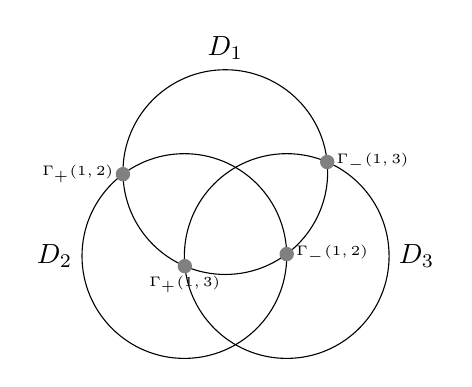
\begin{tikzpicture}[scale=1.3]
%\draw [help lines] (-5,-3) grid (5,3);

\draw[name path = c1] (0,0) circle (1cm);
\draw[name path = c3] (0.6,-0.82) circle (1cm);
\draw[name path = c2] (-0.4,-0.82) circle (1cm);

\node[above] at (0, 1) {$D_1$};
\node[left] at (-1.4, -0.82) {$D_2$};
\node[right] at (1.6, -0.82) {$D_3$};

\path [name intersections={of=c1 and c3}] ;
\foreach \i in {1,...,2}
\fill [color=gray] (intersection-\i) circle (2pt) ;

\node[right] at (intersection-1) {\tiny $\Gamma_-(1,3)$};
\node[left, below] at (intersection-2) {\tiny $\Gamma_+(1,3)$};

\path [name intersections={of=c1 and c2}] ;
\foreach \i in {1,...,2}
\fill [color=gray] (intersection-\i) circle (2pt) ;

\node[left] at (intersection-1) {\tiny $\Gamma_+(1,2)$};
\node[below,right] at (intersection-2) {\tiny $\Gamma_-(1,2)$};

%\draw [-] (-5,0) -- (5,0);
%\draw [-] (0,-3) -- (0,3);
%\draw [|-|] (0.001,-0.1) -- (4.999,-0.1);
\end{tikzpicture}
		\source{Elaborated by the author.}
		\label{fig:3disks_intersect}
	\end{figure}
\end{frame}


\begin{frame}{Maximum Weight Clique Problem}{Algorithm}
	
	Some observations allow us to arrive at the algorithm:
	
%	For a disk $D_i$, a counter-clockwise traversal visits every $\Gamma_+(i,j)$ and $\Gamma_-(i,j)$ in counter-clockwise order.
	
	\begin{itemize}
		\item An intersection region of disks is bounded by arcs.
		
		\item The arc $A(\Gamma_+(i,j),\Gamma_-(i,j))$ (counter-clockwise) determines a region where $i$ and $j$ intersect.
		

		\item For every disk $D_i$, we want to find an angle $\theta$, such that $$w(\{D_k : \theta \in A(\Gamma_+(i,k),\Gamma_-(i,k))\}),$$ is maximized. Most overlapping intervals (circular).
		
		\item To transform it to the problem of finding the most overlapping intervals, just copy the list of intersection angles. The arcs such that $\Gamma_+(i,j) > \Gamma_-(i,j)$ will be considered.
	\end{itemize}
\end{frame}

\begin{frame}{Maximum Weight Clique Problem}{Algorithm}
	
	Transforming it to the most overlapping intervals.
	
	\begin{figure}[H]
		\centering
		
		\caption{The intersections list of a disk with three other disks.}
		\input{figures/fig:array_disks.tex}
		\source{Elaborated by the author.}
		%\label{fig:array_disks}
	\end{figure}
\end{frame}

\begin{frame}{Maximum Weight Clique Problem}{Algorithm}
	Our algorithm for the Maximum Weight Clique Problem:\\~\\
	
	For every disk $D_i$, do:
	\begin{itemize}
		\item Get the sorted list of intersection angles with $D_i$
				$A=\cap_{j}\Gamma_+(i,j) \cup \Gamma_-(i,j)$.
		\item Traverse it twice starting at the angle with smallest value.
		\begin{itemize}
			\item Keep a set of active disks. When an opening angle is visited, make the disk active, otherwise remove it from the set.
			\item Update the optimal solution. Use the closing angle.
		\end{itemize}
	\end{itemize}
\end{frame}


%\begin{frame}{Maximum Weight Clique Problem}{Algorithm}
%\begin{figure}
	%\centering
	
%	\caption{A traversal for $D_1$ with green disks representing the active set and red signs representing the current angle being visited (some are omitted).}
%	\input{figures/mcd_sim.tex}
%		\source{Elaborated by the author.}
	%\label{fig:array_disks}
%\end{figure}
%\end{frame}

\begin{frame}{Maximum Weight Clique Problem}{Algorithm}

	\begin{figure}
		\caption{A traversal for $D_1$ with green disks representing the active set and red signs representing the current angle being visited (some are omitted).}
		\only<1>{\input{figures/mcd_sim_1.tex}}
		\only<2>{\input{figures/mcd_sim_2.tex}}
		\only<3>{\input{figures/mcd_sim_2_5.tex}}
		\only<4>{\input{figures/mcd_sim_3.tex}}
		\only<5>{\input{figures/mcd_sim_4.tex}}
		\only<6>{\input{figures/mcd_sim_5.tex}}
		\only<7>{\input{figures/mcd_sim_6.tex}}
		\only<8>{\tikzset{every picture/.style={line width=0.75pt}} %set default line width to 0.75pt        

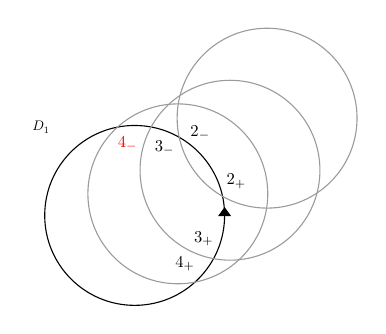
\begin{tikzpicture}[x=1pt,y=1pt,yscale=-1.3,xscale=1.3]
%uncomment if require: \path (0,95); %set diagram left start at 0, and has height of 95

%Shape: Circle [id:dp37777408295388804] 
\draw   (21,59.5) .. controls (21,45.69) and (32.19,34.5) .. (46,34.5) .. controls (59.81,34.5) and (71,45.69) .. (71,59.5) .. controls (71,73.31) and (59.81,84.5) .. (46,84.5) .. controls (32.19,84.5) and (21,73.31) .. (21,59.5) -- cycle ;


%Shape: Circle [id:dp4562198988843913] 
\draw  [color={rgb, 255:red, 155; green, 155; blue, 155 },draw opacity=1 ] (47.5,46.94) .. controls (47.5,33.14) and (58.69,21.94) .. (72.5,21.94) .. controls (86.31,21.94) and (97.5,33.14) .. (97.5,46.94) .. controls (97.5,60.75) and (86.31,71.94) .. (72.5,71.94) .. controls (58.69,71.94) and (47.5,60.75) .. (47.5,46.94) -- cycle ;


%Shape: Circle [id:dp8913971633985722] 
\draw  [color={rgb, 255:red, 155; green, 155; blue, 155 } ,draw opacity=1 ] (33,53.5) .. controls (33,39.69) and (44.19,28.5) .. (58,28.5) .. controls (71.81,28.5) and (83,39.69) .. (83,53.5) .. controls (83,67.31) and (71.81,78.5) .. (58,78.5) .. controls (44.19,78.5) and (33,67.31) .. (33,53.5) -- cycle ;


%Shape: Circle [id:dp05970043129919356] 
\draw  [color={rgb, 255:red, 155; green, 155; blue, 155 }  ,draw opacity=1 ] (57.81,32.47) .. controls (57.81,18.66) and (69,7.47) .. (82.81,7.47) .. controls (96.62,7.47) and (107.81,18.66) .. (107.81,32.47) .. controls (107.81,46.27) and (96.62,57.47) .. (82.81,57.47) .. controls (69,57.47) and (57.81,46.27) .. (57.81,32.47) -- cycle ;
%Straight Lines [id:da04725899028195979] 
%\draw[densely dotted]  (21,59.5) -- (71,59.5) ;


%Flowchart: Extract [id:dp5267407418119328] 
\draw  [fill={rgb, 255:red, 0; green, 0; blue, 0 }  ,fill opacity=1 ] (71,57.45) -- (72.52,59.55) -- (69.48,59.55) -- cycle ;

\draw (60,73) node [scale=0.6]  {$4_+$};
% Text Node
\draw (65.22,66) node [scale=0.6]  {$3_+$};
% Text Node
\draw (74.22,50) node [scale=0.6]  {$2_+$};
% Text Node
\draw (64.22,36.56) node [scale=0.6]  {$2_-$};
% Text Node
\draw (54.32,40.66) node [scale=0.6]  {$3_-$};
% Text Node
\draw (44.02,39.56) node [scale=0.6,color=red]  {$4_-$};


% Text Node
\draw (20,35) node [scale=0.5]  {$D_{1}$};
\end{tikzpicture}

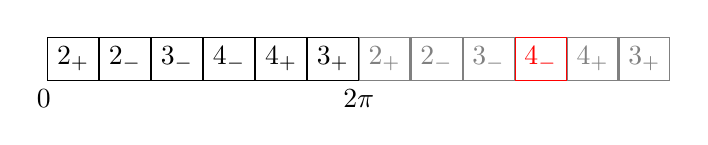
\begin{tikzpicture}

\matrix [matrix of nodes,row sep=,row sep=0mm,
column 1/.style={nodes={rectangle,draw,minimum width=1.5em, minimum height=0.5em}},
column 2/.style={nodes={rectangle,draw,minimum width=1.5em, minimum height=0.5em}},
column 3/.style={nodes={rectangle,draw,minimum width=1.5em, minimum height=0.5em}},
column 4/.style={nodes={rectangle,draw,minimum width=1.5em, minimum height=0.5em}},
column 5/.style={nodes={rectangle,draw,minimum width=1.5em, minimum height=0.5em}},
column 6/.style={nodes={rectangle,draw,minimum width=1.5em, minimum height=0.5em}},
column 7/.style={nodes={rectangle,draw,minimum width=1.5em, color=gray, minimum height=0.5em}},
column 8/.style={nodes={rectangle,draw,minimum width=1.5em, color=gray, minimum height=0.5em}},
column 9/.style={nodes={rectangle,draw,minimum width=1.5em, color=gray, minimum height=0.5em}},
column 10/.style={nodes={rectangle,draw,minimum width=1.5em, color=red, minimum height=0.5em}},
column 11/.style={nodes={rectangle,draw,minimum width=1.5em, color=gray, minimum height=0.5em}},
column 12/.style={nodes={rectangle,draw,minimum width=1.5em, color=gray, minimum height=0.5em}}
] (O)
{
$2_+$ & $2_-$ & $3_-$ & $4_-$ & $4_+$ & $3_+$ & $2_+$ & $2_-$ & $3_-$ & $4_-$ & $4_+$ & $3_+$\\
	%$+$ & $-$ & $-$ & $-$ & $+$ & $+$\\
};

\node at (-4,-0.5) {$0$};
\node at (0,-0.5) {$2\pi$};
\end{tikzpicture}}
			\source{Elaborated by the author.}
	\end{figure}
\end{frame}


\begin{frame}{Maximum Weight Clique Problem}{Algorithm}
	
	The run-time complexity of the algorithm is $\bigO(n^2\log{n})$.
	
	\begin{itemize}
		\item There are $\bigO(n^2)$ intersections among $n$ disks.
		
		\item Sorting takes $\bigO(n^2\log{n})$.
		
		\item The traversal takes $\bigO(n)$ for every disk.
		
		\item It can be implemented in $K\log{n}$ where $K$ is the number of intersections \autocite{bentley:1979}.
		
		\item The algorithm is basically finding the most number of overlapping intervals $n$ times.
		
		\item As it was mentioned, the solution found by this algorithm is a solution for the Maximal Covering by One Disk.
	\end{itemize}

\end{frame}

\begin{frame}{Maximum Covering by Disks}{Multiple disks}
	
	Works found in the literature:
	
	\begin{itemize}
		\item In \autocite{cabello:2006} a $\bigO(n^{2m-1})$ algorithm was proposed. Also a $(1-\epsilon)-$approximation that runs in $\bigO(n\log{n})$ was introduced.
		
		\item In \autocite{zhou} a heuristic method using an algorithm called mean-shift was developed. The mean-shift algorithm converges to a local density maxima of any probability distribution and it is used to find a smaller candidate list of centers for the disks.
	\end{itemize}
	
	Because of the similarities, we will discuss only the multiple ellipses algorithm later.
	
\end{frame}
\section{Maximal Covering by Ellipses}

\begin{frame}{Ellipses}
	
	\begin{block}{Ellipse}
		Given a center $c \in \R^2$ and $Q \in \R^ {2x2}$, an ellipse is the set of points that satisfy
		
		\begin{equation*}
		||u-c||_Q^2 = (u-c)^TQ(u-c) = 1,
		\end{equation*}
		
		with $\le$ representing the set of covered points.
	\end{block}
	
	\begin{block}{Axis-parallel ellipse}
		Any $2$ by $2$ diagonal d.p. matrix determines an axis-parallel ellipse, which can also be described by
		
		\begin{equation*}
		\frac{(x-c_x)^2}{a^2} + \frac{(y-c_y)^2}{b^2} = 1,
		\end{equation*}
		
		where $(a,b)$ are the shape parameters and $c=(c_x,c_y)$ is the center.
	\end{block}
	
\end{frame}

\begin{frame}{Ellipses}
	\begin{figure}[H]
		\centering
		
		\caption{The ellipse seen as just a linear transformation of a circle.}
		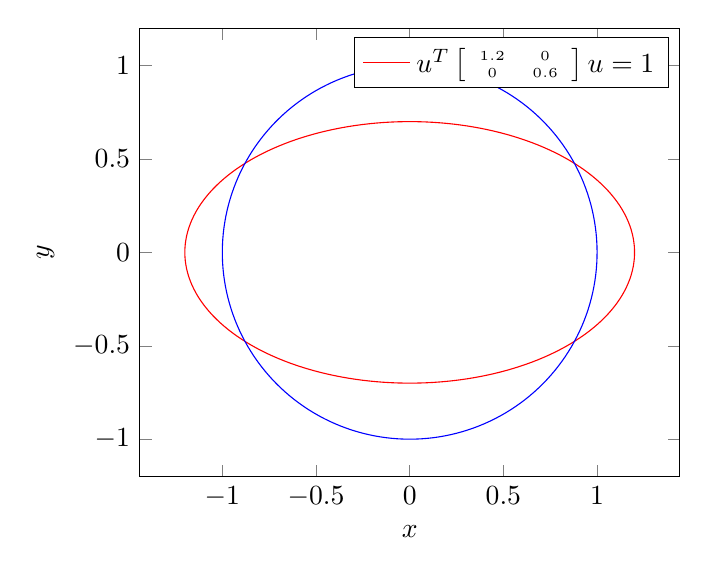
\begin{tikzpicture}
\begin{axis}[
    %axis lines = left,
    xlabel = $x$,
    ylabel = {$y$},
]
%Below the red parabola is defined
\addplot [domain=-pi:pi,samples=200,red]({1.2*cos(deg(x))}, {0.7*sin(deg(x))});

\addlegendentry{$\tiny u^T\left[\begin{array}{cc}
		1.2 & 0\\
		0 & 0.6
	\end{array}\right]u = 1$}
\addplot [domain=-pi:pi,samples=200,blue]({sin(deg(x))}, {cos(deg(x))});
\end{axis}
\end{tikzpicture}
		\source{Elaborated by the author.}
		\label{fig:3ellipses_intersect}
		
	\end{figure}
\end{frame}



\begin{frame}{Maximal Covering by Ellipses}{One ellipse}
	Let $MCE(\Pp, a, b)$ be an instance of the maximal covering by one ellipse, with $E$ being an ellipse with shape parameters $(a,b) \in \R_{>0}^2$, and $\Pp=\{p_1,\dots,p_n\}$ is a set of $n$ points with each point having a positive weight $w_i$, an optimal solution of $MCE(\Pp, a, b)$ is given by
	
	\begin{equation*}
	\max_q w(\Pp \cap E(q)),
	\end{equation*}

	\begin{itemize}
		\item $E(q)$ is an axis-parallel ellipse with center point $q$.
		\item $w(A)$, $A \subset \Pp$, is the sum of the weights of every point in $\Pp$.
		\item Same algorithm for one disk.
	\end{itemize}

\end{frame}

\begin{frame}{Maximal Covering by Ellipses}{One ellipse}
\begin{figure}[H]
	\centering
	
	\caption{Intersection points of $E_1$ with $E_2$ and $E_3$ along with opening and closing angles indicators.}
	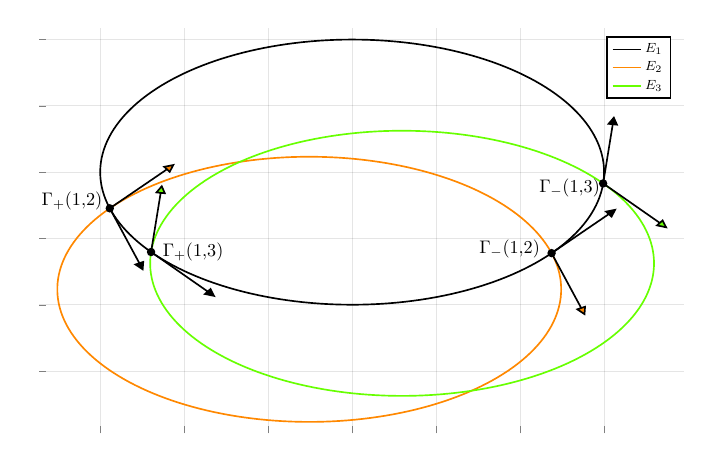
\begin{tikzpicture}[scale=0.6]
\begin{axis}[height = {101.6mm}, ylabel = {}, xmin = {-3.7279015473763786}, xmax = {3.956162987575968}, ymax = {2.172965670438345}, xlabel = {}, unbounded coords=jump,scaled x ticks = false,xlabel style = {font = {\fontsize{11 pt}{14.3 pt}\selectfont}, color = {rgb,1:red,0.00000000;green,0.00000000;blue,0.00000000}, draw opacity = 1.0, rotate = 0.0},xmajorgrids = true,xtick = {-3.0,-2.0,-1.0,0.0,1.0,2.0,3.0},xticklabels = {},xtick align = inside,xticklabel style = {font = {\fontsize{8 pt}{10.4 pt}\selectfont}, color = {rgb,1:red,0.00000000;green,0.00000000;blue,0.00000000}, draw opacity = 1.0, rotate = 0.0},x grid style = {color = {rgb,1:red,0.00000000;green,0.00000000;blue,0.00000000},
draw opacity = 0.1,
line width = 0.5,
solid},axis lines* = left,separate axis lines,x axis line style = {draw opacity = 0},scaled y ticks = false,ylabel style = {font = {\fontsize{11 pt}{14.3 pt}\selectfont}, color = {rgb,1:red,0.00000000;green,0.00000000;blue,0.00000000}, draw opacity = 1.0, rotate = 0.0},ymajorgrids = true,ytick = {-3.0,-2.0,-1.0,0.0,1.0,2.0},yticklabels = {},ytick align = inside,yticklabel style = {font = {\fontsize{8 pt}{10.4 pt}\selectfont}, color = {rgb,1:red,0.00000000;green,0.00000000;blue,0.00000000}, draw opacity = 1.0, rotate = 0.0},y grid style = {color = {rgb,1:red,0.00000000;green,0.00000000;blue,0.00000000},
draw opacity = 0.1,
line width = 0.5,
solid},axis lines* = left,separate axis lines,y axis line style = {draw opacity = 0},    xshift = 0.0mm,
    yshift = 0.0mm,
    axis background/.style={fill={rgb,1:red,1.00000000;green,1.00000000;blue,1.00000000}}
,legend style = {color = {rgb,1:red,0.00000000;green,0.00000000;blue,0.00000000},
draw opacity = 1.0,
line width = 1,
solid,fill = {rgb,1:red,1.00000000;green,1.00000000;blue,1.00000000},font = {\fontsize{8 pt}{10.4 pt}\selectfont}},colorbar style={title=}, ymin = {-3.9406895045294608}, width = {152.4mm}]\addplot+ [color = {rgb,1:red,0.00000000;green,0.00000000;blue,0.00000000},
draw opacity = 1.0,
line width = 1,
solid,mark = none,
mark size = 2.0,
mark options = {
    color = {rgb,1:red,0.00000000;green,0.00000000;blue,0.00000000}, draw opacity = 1.0,
    fill = {rgb,1:red,0.00000000;green,0.00000000;blue,0.00000000}, fill opacity = 1.0,
    line width = 1,
    rotate = 0,
    solid
}]coordinates {
(3.0, 0.0)
(2.9985047673785212, 0.06313709952962106)
(2.99402055999448, 0.1262112626253473)
(2.9865518478033177, 0.18915961558968988)
(2.9761060757797733, 0.2519194101354351)
(2.962693656496571, 0.31442808593450156)
(2.9463279597449414, 0.37662333297943573)
(2.9270252992073207, 0.43844315369538267)
(2.9048049161955216, 0.4998259247406167)
(2.879688960470571, 0.5607104584340288)
(2.8517024681633485, 0.6210360637483376)
(2.8208733368180265, 0.6807426068082256)
(2.787232297583192, 0.7397705708330936)
(2.7508128845783664, 0.7980611154646818)
(2.7116514014664705, 0.8555561354204192)
(2.669786885265541, 0.9121983184140319)
(2.625261067435781, 0.9679312022856775)
(2.578118332280736, 1.0226992312846535)
(2.528405672704052, 1.076447811448577)
(2.4761726433659286, 1.1291233650238361)
(2.421471311285956, 1.1806733838730568)
(2.3643562039415773, 1.2310464818163585)
(2.3048842549139126, 1.2801924458542142)
(2.2431147471351274, 1.3280622862208624)
(2.1791092537939183, 1.3746082852183685)
(2.1129315769580166, 1.4197840447826657)
(2.0446476839749015, 1.4635445327341534)
(1.974325641714113, 1.505846127666754)
(1.902035548716716, 1.546646662430678)
(1.82784946531955, 1.5859054661655572)
(1.7518413418239187, 1.6235834048420414)
(1.6740869447803206, 1.6596429202714515)
(1.5946637814627043, 1.6940480675445977)
(1.5136510226075326, 1.7267645508624465)
(1.4311294234946685, 1.7577597577229207)
(1.3471812434487604, 1.7870027914297482)
(1.261890163841353, 1.8144645018909626)
(1.1753412046754794, 1.840117514676349)
(1.0876206398358734, 1.8639362583048695)
(0.9988159110892831, 1.885896989734874)
(0.9090155409206182, 1.9059778180316784)
(0.8183090442918096, 1.9241587261889257)
(0.7267868394113495, 1.9404215910819727)
(0.6345401576034572, 1.9547502015334144)
(0.541660952366707, 1.9671302744727397)
(0.4482418077127828, 1.9775494691740052)
(0.35437584587672416, 1.9859973995573392)
(0.26015663449065285, 1.9924656445420135)
(0.1656780933135245, 1.9969477564407576)
(0.0710344006098723, 1.9994392673869559)
(-0.02368010072913993, 1.9999376937883127)
(-0.1183709972287581, 1.9984425388025513)
(-0.21294389894404733, 1.9949552928326777)
(-0.3073045335498399, 1.9894794320413138)
(-0.40135884031343716, 1.9820204148855842)
(-0.49501306385639726, 1.9725856766760055)
(-0.588173847611934, 1.9611846221648082)
(-0.68074832688477, 1.9478286161710756)
(-0.7726442214206901, 1.9325309722520436)
(-0.8637699273934991, 1.9153069394318591)
(-0.9540346087177143, 1.896173687001019)
(-1.043348287595947, 1.8751502874016501)
(-1.1316219342107279, 1.8522576972156826)
(-1.2187675554713666, 1.8275187362748735)
(-1.304698282727379, 1.8009580649135033)
(-1.389328458361043, 1.7726021593864174)
(-1.4725737211727805, 1.7424792854769193)
(-1.5543510904742317, 1.710619470320824)
(-1.6345790488052114, 1.6770544724747547)
(-1.713177623192084, 1.6418177502585252)
(-1.7900684648665677, 1.604944428403156)
(-1.8651749273654852, 1.566471263037781)
(-1.9384221429336286, 1.5264366050503373)
(-2.009737097153566, 1.484880361858566)
(-2.079048701727995, 1.4418439576294326)
(-2.1462878653421136, 1.3973702919866131)
(-2.2113875625353363, 1.3515036972472176)
(-2.274282900513736, 1.3042898942303736)
(-2.3349111838365904, 1.2557759466817167)
(-2.393211976912558, 1.206010214359229)
(-2.449127164243197, 1.1550423048271772)
(-2.502601008353752, 1.1029230240062151)
(-2.5535802053534837, 1.0497043255289369)
(-2.6020139380701437, 0.9954392589513668)
(-2.6478539267056407, 0.9401819168720059)
(-2.6910544769623908, 0.8839873810111583)
(-2.7315725255923864, 0.8269116673042683)
(-2.7693676833235816, 0.769011670064022)
(-2.8044022751207947, 0.7103451052668572)
(-2.8366413777410013, 0.6509704530204232)
(-2.8660528545455843, 0.5909468992693401)
(-2.8926073875348353, 0.5303342767973575)
(-2.916278506572771, 0.46919300558473775)
(-2.9370426157731435, 0.4075840325803047)
(-2.954879017020331, 0.3455687709481997)
(-2.9697699306016716, 0.28320903884990317)
(-2.9817005129306633, 0.22056699782255015)
(-2.9906588713433795, 0.1577050908149532)
(-2.996636075953331, 0.09468597994311641)
(-2.9996261685529717, 0.03157248402727453)
(-2.9996261685529717, -0.031572484027274035)
(-2.996636075953331, -0.09468597994311592)
(-2.9906588713433795, -0.1577050908149527)
(-2.9817005129306637, -0.22056699782254965)
(-2.9697699306016716, -0.2832090388499027)
(-2.9548790170203314, -0.34556877094819927)
(-2.9370426157731435, -0.40758403258030423)
(-2.916278506572771, -0.46919300558473725)
(-2.8926073875348353, -0.530334276797357)
(-2.866052854545585, -0.5909468992693396)
(-2.8366413777410013, -0.6509704530204228)
(-2.804402275120795, -0.7103451052668568)
(-2.769367683323582, -0.7690116700640215)
(-2.7315725255923864, -0.8269116673042679)
(-2.6910544769623908, -0.8839873810111578)
(-2.647853926705641, -0.9401819168720055)
(-2.6020139380701437, -0.9954392589513663)
(-2.5535802053534837, -1.0497043255289367)
(-2.5026010083537527, -1.1029230240062147)
(-2.4491271642431975, -1.155042304827177)
(-2.393211976912559, -1.2060102143592286)
(-2.3349111838365904, -1.2557759466817162)
(-2.274282900513737, -1.3042898942303731)
(-2.211387562535337, -1.3515036972472174)
(-2.1462878653421145, -1.3973702919866127)
(-2.079048701727996, -1.4418439576294324)
(-2.0097370971535664, -1.4848803618585658)
(-1.9384221429336304, -1.5264366050503364)
(-1.8651749273654858, -1.5664712630377808)
(-1.7900684648665695, -1.604944428403155)
(-1.713177623192085, -1.641817750258525)
(-1.634579048805211, -1.677054472474755)
(-1.5543510904742333, -1.7106194703208233)
(-1.4725737211727812, -1.742479285476919)
(-1.389328458361045, -1.7726021593864167)
(-1.3046982827273796, -1.800958064913503)
(-1.2187675554713666, -1.8275187362748735)
(-1.131621934210729, -1.8522576972156821)
(-1.0433482875959472, -1.8751502874016501)
(-0.9540346087177163, -1.8961736870010186)
(-0.8637699273935, -1.915306939431859)
(-0.7726442214206894, -1.9325309722520438)
(-0.6807483268847714, -1.9478286161710754)
(-0.5881738476119341, -1.9611846221648082)
(-0.4950130638563993, -1.9725856766760053)
(-0.4013588403134378, -1.9820204148855842)
(-0.3073045335498393, -1.989479432041314)
(-0.2129438989440487, -1.9949552928326775)
(-0.11837099722875816, -1.9984425388025513)
(-0.023680100729141333, -1.9999376937883127)
(0.07103440060987157, -1.9994392673869559)
(0.1656780933135251, -1.9969477564407576)
(0.2601566344906514, -1.9924656445420135)
(0.3543758458767241, -1.9859973995573392)
(0.44824180771278144, -1.9775494691740052)
(0.5416609523667063, -1.96713027447274)
(0.6345401576034577, -1.9547502015334144)
(0.7267868394113488, -1.9404215910819727)
(0.8183090442918095, -1.9241587261889257)
(0.9090155409206169, -1.9059778180316789)
(0.998815911089283, -1.885896989734874)
(1.0876206398358716, -1.8639362583048702)
(1.1753412046754788, -1.840117514676349)
(1.261890163841353, -1.8144645018909626)
(1.3471812434487593, -1.7870027914297486)
(1.4311294234946685, -1.7577597577229207)
(1.5136510226075308, -1.7267645508624474)
(1.5946637814627036, -1.694048067544598)
(1.6740869447803208, -1.6596429202714515)
(1.7518413418239178, -1.6235834048420419)
(1.82784946531955, -1.5859054661655572)
(1.9020355487167147, -1.546646662430679)
(1.9743256417141124, -1.5058461276667543)
(2.044647683974902, -1.4635445327341534)
(2.1129315769580157, -1.4197840447826664)
(2.179109253793918, -1.3746082852183685)
(2.243114747135126, -1.3280622862208633)
(2.3048842549139117, -1.2801924458542147)
(2.3643562039415773, -1.231046481816358)
(2.4214713112859556, -1.1806733838730574)
(2.4761726433659286, -1.1291233650238361)
(2.528405672704051, -1.076447811448578)
(2.5781183322807357, -1.0226992312846537)
(2.6252610674357815, -0.9679312022856771)
(2.66978688526554, -0.9121983184140325)
(2.7116514014664705, -0.8555561354204191)
(2.750812884578366, -0.7980611154646828)
(2.7872322975831914, -0.7397705708330939)
(2.820873336818026, -0.680742606808227)
(2.8517024681633485, -0.6210360637483382)
(2.879688960470571, -0.5607104584340287)
(2.904804916195521, -0.4998259247406176)
(2.9270252992073207, -0.4384431536953829)
(2.946327959744941, -0.37662333297943695)
(2.9626936564965707, -0.3144280859345021)
(2.9761060757797737, -0.25191941013543495)
(2.9865518478033177, -0.18915961558969077)
(2.99402055999448, -0.12621126262534743)
(2.9985047673785212, -0.06313709952962226)
(3.0, -4.898587196589413e-16)
};
\addlegendentry{$E_1$}
\addplot+ [color = {rgb,1:red,1.00000000;green,0.53160000;blue,0.00000000},
draw opacity = 1.0,
line width = 1,
solid,mark = none,
mark size = 2.0,
mark options = {
    color = {rgb,1:red,0.00000000;green,0.00000000;blue,0.00000000}, draw opacity = 1.0,
    fill = {rgb,1:red,1.00000000;green,0.53160000;blue,0.00000000}, fill opacity = 1.0,
    line width = 1,
    rotate = 0,
    solid
}]coordinates {
(2.489198145750716, -1.7677238340911159)
(2.487702913129237, -1.704586734561495)
(2.483218705745196, -1.6415125714657686)
(2.4757499935540337, -1.578564218501426)
(2.4653042215304892, -1.5158044239556807)
(2.451891802247287, -1.4532957481566142)
(2.4355261054956574, -1.3911005011116802)
(2.4162234449580366, -1.3292806803957333)
(2.3940030619462376, -1.2678979093504992)
(2.368887106221287, -1.207013375657087)
(2.3409006139140645, -1.1466877703427782)
(2.3100714825687425, -1.0869812272828903)
(2.2764304433339078, -1.0279532632580222)
(2.2400110303290823, -0.969662718626434)
(2.2008495472171865, -0.9121676986706967)
(2.158985031016257, -0.855525515677084)
(2.114459213186497, -0.7997926318054384)
(2.067316478031452, -0.7450246028064624)
(2.0176038184547678, -0.691276022642539)
(1.9653707891166445, -0.6386004690672797)
(1.910669457036672, -0.5870504502180591)
(1.8535543496922933, -0.5366773522747574)
(1.7940824006646285, -0.4875313882369017)
(1.7323128928858433, -0.43966154787025347)
(1.6683073995446343, -0.39311554887274736)
(1.6021297227087326, -0.34793978930845015)
(1.5338458297256174, -0.3041793013569625)
(1.4635237874648293, -0.2618777064243618)
(1.3912336944674322, -0.22107717166043783)
(1.317047611070266, -0.18181836792555872)
(1.2410394875746347, -0.14414042924907444)
(1.1632850905310366, -0.10808091381966434)
(1.0838619272134205, -0.0736757665465182)
(1.0028491683582486, -0.040959283228669374)
(0.9203275692453846, -0.009964076368195185)
(0.8363793891994765, 0.019278957338632274)
(0.7510883095920692, 0.04674066779984676)
(0.6645393504261955, 0.07239368058523321)
(0.5768187855865895, 0.09621242421375364)
(0.4880140568399992, 0.11817315564375819)
(0.3982136866713343, 0.13825398394056254)
(0.3075071900425257, 0.1564348920978098)
(0.21598498516206555, 0.17269775699085677)
(0.12373830335417324, 0.1870263674422985)
(0.030859098117423045, 0.1994064403816238)
(-0.0625600465365011, 0.20982563508288932)
(-0.15642600837255977, 0.21827356546622334)
(-0.2506452197586311, 0.22474181045089758)
(-0.3451237609357594, 0.22922392234964173)
(-0.4397674536394116, 0.23171543329584)
(-0.5344819549784239, 0.23221385969719677)
(-0.629172851478042, 0.2307187047114354)
(-0.7237457531933312, 0.2272314587415618)
(-0.8181063877991238, 0.22175559795019795)
(-0.9121606945627211, 0.21429658079446834)
(-1.0058149181056812, 0.2048618425848896)
(-1.0989757018612178, 0.19346078807369227)
(-1.1915501811340539, 0.18010478207995972)
(-1.283446075669974, 0.16480713816092774)
(-1.374571781642783, 0.14758310534074326)
(-1.464836462966998, 0.12844985290990318)
(-1.554150141845231, 0.10742645331053424)
(-1.642423788460012, 0.08453386312456668)
(-1.7295694097206504, 0.0597949021837576)
(-1.815500136976663, 0.03323423082238741)
(-1.9001303126103268, 0.004878325295301522)
(-1.9833755754220643, -0.02524454861419656)
(-2.0651529447235157, -0.05710436377029193)
(-2.1453809030544955, -0.09066936161636119)
(-2.223979477441368, -0.12590608383259072)
(-2.3008703191158517, -0.1627794056879599)
(-2.375976781614769, -0.20125257105333483)
(-2.4492239971829126, -0.2412872290407786)
(-2.52053895140285, -0.2828434722325499)
(-2.589850555977279, -0.32587987646168326)
(-2.6570897195913976, -0.3703535421045028)
(-2.7221894167846203, -0.41622013684389825)
(-2.78508475476302, -0.4634339398607423)
(-2.8457130380858744, -0.5119478874093992)
(-2.904013831161842, -0.5617136197318868)
(-2.959929018492481, -0.6126815292639387)
(-3.0134028626030362, -0.6648008100849008)
(-3.0643820596027678, -0.718019508562179)
(-3.1128157923194277, -0.7722845751397491)
(-3.1586557809549247, -0.82754191721911)
(-3.201856331211675, -0.8837364530799576)
(-3.2423743798416704, -0.9408121667868475)
(-3.2801695375728657, -0.9987121640270938)
(-3.3152041293700787, -1.0573787288242587)
(-3.3474432319902854, -1.1167533810706927)
(-3.3768547087948684, -1.1767769348217758)
(-3.4034092417841193, -1.2373895572937585)
(-3.427080360822055, -1.2985308285063781)
(-3.4478444700224276, -1.3601398015108113)
(-3.465680871269615, -1.4221550631429163)
(-3.4805717848509556, -1.4845147952412128)
(-3.4925023671799473, -1.5471568362685657)
(-3.5014607255926635, -1.6100187432761626)
(-3.507437930202615, -1.6730378541479995)
(-3.5104280228022557, -1.7361513500638415)
(-3.5104280228022557, -1.7992963181183899)
(-3.507437930202615, -1.8624098140342318)
(-3.5014607255926635, -1.9254289249060685)
(-3.4925023671799478, -1.9882908319136656)
(-3.4805717848509556, -2.0509328729410186)
(-3.4656808712696154, -2.113292605039315)
(-3.4478444700224276, -2.17530786667142)
(-3.427080360822055, -2.236916839675853)
(-3.4034092417841193, -2.298058110888473)
(-3.376854708794869, -2.3586707333604555)
(-3.3474432319902854, -2.4186942871115384)
(-3.315204129370079, -2.4780689393579727)
(-3.280169537572866, -2.5367355041551374)
(-3.2423743798416704, -2.5946355013953837)
(-3.201856331211675, -2.6517112151022735)
(-3.158655780954925, -2.7079057509631212)
(-3.1128157923194277, -2.763163093042482)
(-3.0643820596027678, -2.8174281596200528)
(-3.0134028626030367, -2.870646858097331)
(-2.9599290184924816, -2.922766138918293)
(-2.904013831161843, -2.9737340484503445)
(-2.8457130380858744, -3.0234997807728323)
(-2.785084754763021, -3.072013728321489)
(-2.7221894167846212, -3.1192275313383333)
(-2.6570897195913985, -3.1650941260777286)
(-2.58985055597728, -3.2095677917205485)
(-2.5205389514028504, -3.2526041959496816)
(-2.4492239971829144, -3.2941604391414523)
(-2.37597678161477, -3.3341950971288967)
(-2.3008703191158535, -3.3726682624942708)
(-2.223979477441369, -3.4095415843496406)
(-2.145380903054495, -3.444778306565871)
(-2.065152944723517, -3.478343304411939)
(-1.9833755754220652, -3.510203119568035)
(-1.900130312610329, -3.5403259934775324)
(-1.8155001369766635, -3.568681899004619)
(-1.7295694097206504, -3.5952425703659894)
(-1.6424237884600128, -3.619981531306798)
(-1.554150141845231, -3.642874121492766)
(-1.4648364629670003, -3.6638975210921343)
(-1.3745717816427838, -3.683030773522975)
(-1.2834460756699735, -3.7002548063431595)
(-1.1915501811340552, -3.7155524502621913)
(-1.098975701861218, -3.7289084562559243)
(-1.0058149181056832, -3.740309510767121)
(-0.9121606945627218, -3.7497442489767003)
(-0.8181063877991233, -3.75720326613243)
(-0.7237457531933327, -3.7626791269237936)
(-0.6291728514780421, -3.766166372893667)
(-0.5344819549784252, -3.7676615278794285)
(-0.4397674536394124, -3.7671631014780718)
(-0.3451237609357588, -3.7646715905318735)
(-0.2506452197586325, -3.760189478633129)
(-0.15642600837255982, -3.753721233648455)
(-0.06256004653650249, -3.745273303265121)
(0.03085909811742238, -3.734854108563856)
(0.1237383033541738, -3.72247403562453)
(0.21598498516206488, -3.7081454251730888)
(0.3075071900425256, -3.6918825602800416)
(0.39821368667133294, -3.6737016521227948)
(0.4880140568399991, -3.6536208238259897)
(0.5768187855865877, -3.631660092395986)
(0.6645393504261948, -3.607841348767465)
(0.7510883095920692, -3.5821883359820785)
(0.8363793891994754, -3.5547266255208645)
(0.9203275692453846, -3.5254835918140364)
(1.0028491683582468, -3.4944883849535633)
(1.0838619272134196, -3.461771901635714)
(1.163285090531037, -3.427366754362567)
(1.2410394875746338, -3.391307238933158)
(1.317047611070266, -3.353629300256673)
(1.3912336944674308, -3.3143704965217946)
(1.4635237874648284, -3.27356996175787)
(1.533845829725618, -3.2312683668252693)
(1.6021297227087317, -3.1875078788737823)
(1.6683073995446338, -3.1423321193094846)
(1.732312892885842, -3.0957861203119794)
(1.7940824006646277, -3.0479162799453308)
(1.8535543496922933, -2.998770315907474)
(1.9106694570366716, -2.9483972179641733)
(1.9653707891166445, -2.8968471991149523)
(2.017603818454767, -2.844171645539694)
(2.0673164780314517, -2.7904230653757693)
(2.1144592131864974, -2.735655036376793)
(2.158985031016256, -2.6799221525051484)
(2.2008495472171865, -2.623279969511535)
(2.240011030329082, -2.5657849495557987)
(2.2764304433339073, -2.50749440492421)
(2.310071482568742, -2.4484664408993426)
(2.3409006139140645, -2.388759897839454)
(2.368887106221287, -2.3284342925251447)
(2.394003061946237, -2.2675497588317333)
(2.4162234449580366, -2.206166987786499)
(2.435526105495657, -2.1443471670705527)
(2.4518918022472866, -2.082151920025618)
(2.4653042215304897, -2.019643244226551)
(2.4757499935540337, -1.9568834496808067)
(2.483218705745196, -1.8939350967164632)
(2.487702913129237, -1.8308609336207382)
(2.489198145750716, -1.7677238340911163)
};
\addlegendentry{$E_2$}
\addplot+[draw=none, color = {rgb,1:red,0.00000000;green,0.00000000;blue,0.00000000},
draw opacity = 1.0,
line width = 0,
solid,mark = *,
mark size = 2.0,
mark options = {
    color = {rgb,1:red,0.00000000;green,0.00000000;blue,0.00000000}, draw opacity = 1.0,
    fill = {rgb,1:red,0.00000000;green,0.00000000;blue,0.00000000}, fill opacity = 1.0,
    line width = 1,
    rotate = 0,
    solid
},forget plot] coordinates {
(-2.8860343580501877, -0.5460181861659266)
(2.3752325038009037, -1.221705647925189)
};
\addplot+ [color = {rgb,1:red,0.00000000;green,0.00000000;blue,0.00000000},
draw opacity = 1.0,
line width = 1,
solid,mark = none,
mark size = 2.0,
mark options = {
    color = {rgb,1:red,0.00000000;green,0.00000000;blue,0.00000000}, draw opacity = 1.0,
    fill = {rgb,1:red,0.00000000;green,0.00000000;blue,0.00000000}, fill opacity = 1.0,
    line width = 1,
    rotate = 0,
    solid
},fill = {rgb,1:red,0.00000000;green,0.00000000;blue,0.00000000}, fill opacity=1.0,forget plot]coordinates {
(-2.8860343580501877, -0.5460181861659266)
(-2.5335275299915194, -1.3741117413709025)
(-2.4875223324801317, -1.3545280287009764)
(-2.4943601046516672, -1.4661221363936776)
(-2.579532727502907, -1.3936954540408286)
(-2.5335275299915194, -1.3741117413709025)
};
\addplot+ [color = {rgb,1:red,0.00000000;green,0.00000000;blue,0.00000000},
draw opacity = 1.0,
line width = 1,
solid,mark = none,
mark size = 2.0,
mark options = {
    color = {rgb,1:red,0.00000000;green,0.00000000;blue,0.00000000}, draw opacity = 1.0,
    fill = {rgb,1:red,1.00000000;green,0.53160000;blue,0.00000000}, fill opacity = 1.0,
    line width = 1,
    rotate = 0,
    solid
},fill = {rgb,1:red,1.00000000;green,0.53160000;blue,0.00000000}, fill opacity=1.0,forget plot]coordinates {
(-2.8860343580501877, -0.5460181861659266)
(-2.2050451814896377, 0.04241510776583639)
(-2.2377359200414024, 0.08024783979697804)
(-2.1293797174273545, 0.10779658486936561)
(-2.172354442937873, 0.004582375734694735)
(-2.2050451814896377, 0.04241510776583639)
};
\addplot+ [color = {rgb,1:red,0.00000000;green,0.00000000;blue,0.00000000},
draw opacity = 1.0,
line width = 1,
solid,mark = none,
mark size = 2.0,
mark options = {
    color = {rgb,1:red,0.00000000;green,0.00000000;blue,0.00000000}, draw opacity = 1.0,
    fill = {rgb,1:red,0.00000000;green,0.00000000;blue,0.00000000}, fill opacity = 1.0,
    line width = 1,
    rotate = 0,
    solid
},fill = {rgb,1:red,0.00000000;green,0.00000000;blue,0.00000000}, fill opacity=1.0,forget plot]coordinates {
(2.3752325038009037, -1.221705647925189)
(3.0562216803614537, -0.6332723539934262)
(3.023530941809689, -0.5954396219622845)
(3.131887144423737, -0.5678908768898969)
(3.0889124189132184, -0.6711050860245679)
(3.0562216803614537, -0.6332723539934262)
};
\addplot+ [color = {rgb,1:red,0.00000000;green,0.00000000;blue,0.00000000},
draw opacity = 1.0,
line width = 1,
solid,mark = none,
mark size = 2.0,
mark options = {
    color = {rgb,1:red,0.00000000;green,0.00000000;blue,0.00000000}, draw opacity = 1.0,
    fill = {rgb,1:red,1.00000000;green,0.53160000;blue,0.00000000}, fill opacity = 1.0,
    line width = 1,
    rotate = 0,
    solid
},fill = {rgb,1:red,1.00000000;green,0.53160000;blue,0.00000000}, fill opacity=1.0,forget plot]coordinates {
(2.3752325038009037, -1.221705647925189)
(2.7277393318595724, -2.049799203130165)
(2.77374452937096, -2.0302154904602387)
(2.7669067571994246, -2.14180959815294)
(2.6817341343481846, -2.069382915800091)
(2.7277393318595724, -2.049799203130165)
};
\addplot+ [color = {rgb,1:red,0.40530000;green,1.00000000;blue,0.00000000},
draw opacity = 1.0,
line width = 1,
solid,mark = none,
mark size = 2.0,
mark options = {
    color = {rgb,1:red,0.00000000;green,0.00000000;blue,0.00000000}, draw opacity = 1.0,
    fill = {rgb,1:red,0.40530000;green,1.00000000;blue,0.00000000}, fill opacity = 1.0,
    line width = 1,
    rotate = 0,
    solid
}]coordinates {
(3.5948223337290086, -1.375310271633036)
(3.59332710110753, -1.312173172103415)
(3.5888428937234886, -1.2490990090076888)
(3.5813741815323263, -1.1861506560433461)
(3.570928409508782, -1.123390861497601)
(3.5575159902255797, -1.0608821856985347)
(3.54115029347395, -0.9986869386536004)
(3.5218476329363293, -0.9368671179376534)
(3.4996272499245302, -0.8754843468924194)
(3.4745112941995795, -0.8145998131990073)
(3.446524801892357, -0.7542742078846985)
(3.415695670547035, -0.6945676648248105)
(3.3820546313122004, -0.6355397007999425)
(3.345635218307375, -0.5772491561683543)
(3.306473735195479, -0.5197541362126169)
(3.2646092189945497, -0.4631119532190042)
(3.2200834011647896, -0.40737906934735857)
(3.172940666009745, -0.35261104034838264)
(3.1232280064330604, -0.29886246018445917)
(3.070994977094937, -0.24618690660919995)
(3.0162936450149647, -0.19463688775997934)
(2.959178537670586, -0.14426378981667765)
(2.899706588642921, -0.09511782577882189)
(2.837937080864136, -0.047247985412173676)
(2.773931587522927, -0.0007019864146675658)
(2.707753910687025, 0.044473773149629636)
(2.63947001770391, 0.08823426110111732)
(2.5691479754431215, 0.13053585603371798)
(2.4968578824457244, 0.17133639079764196)
(2.4226717990485587, 0.21059519453252107)
(2.3466636755529273, 0.24827313320900535)
(2.268909278509329, 0.28433264863841545)
(2.1894861151917127, 0.3187377959115616)
(2.108473356336541, 0.3514542792294104)
(2.025951757223677, 0.3824494860898846)
(1.9420035771777688, 0.41169251979671206)
(1.8567124975703617, 0.43915423025792655)
(1.7701635384044878, 0.464807243043313)
(1.682442973564882, 0.48862598667183343)
(1.5936382448182917, 0.510586718101838)
(1.5038378746496268, 0.5306675463986423)
(1.4131313780208181, 0.5488484545558896)
(1.321609173140358, 0.5651113194489366)
(1.2293624913324657, 0.5794399299003783)
(1.1364832860957155, 0.5918200028397036)
(1.0430641414417914, 0.6022391975409691)
(0.9491981796057327, 0.6106871279243031)
(0.8549789682196614, 0.6171553729089774)
(0.7605004270425331, 0.6216374848077215)
(0.6658567343388808, 0.6241289957539198)
(0.5711422329998685, 0.6246274221552766)
(0.4764513365002504, 0.6231322671695152)
(0.3818784347849612, 0.6196450211996416)
(0.2875178001791686, 0.6141691604082777)
(0.19346349341557134, 0.6067101432525481)
(0.09980926987261124, 0.5972754050429694)
(0.00664848611707447, 0.5858743505317721)
(-0.08592599315576155, 0.5725183445380395)
(-0.1778218876916816, 0.5572207006190075)
(-0.2689475936644906, 0.539996667798823)
(-0.3592122749887058, 0.520863415367983)
(-0.4485259538669385, 0.49984001576861403)
(-0.5367996004817194, 0.47694742558264647)
(-0.6239452217423581, 0.4522084646418374)
(-0.7098759489983705, 0.4256477932804672)
(-0.7945061246320345, 0.3972918877533813)
(-0.877751387443772, 0.36716901384388323)
(-0.9595287567452232, 0.33530919868778786)
(-1.0397567150762028, 0.3017442008417186)
(-1.1183552894630755, 0.26650747862548907)
(-1.195246131137559, 0.2296341567701199)
(-1.2703525936364768, 0.19116099140474496)
(-1.34359980920462, 0.1511263334173012)
(-1.4149147634245574, 0.10957009022552988)
(-1.4842263679989864, 0.06653368599639653)
(-1.551465531613105, 0.022060020353577015)
(-1.6165652288063277, -0.023806574385818458)
(-1.6794605667847273, -0.07102037740266254)
(-1.7400888501075817, -0.11953432495131944)
(-1.7983896431835493, -0.16930005727380704)
(-1.8543048305141885, -0.22026796680585892)
(-1.9077786746247436, -0.272387247626821)
(-1.9587578716244751, -0.3256059461040992)
(-2.007191604341135, -0.37987101268166934)
(-2.053031592976632, -0.4351283547610302)
(-2.096232143233382, -0.49132289062187784)
(-2.136750191863378, -0.5483986043287677)
(-2.174545349594573, -0.606298601569014)
(-2.209579941391786, -0.6649651663661789)
(-2.2418190440119927, -0.7243398186126129)
(-2.2712305208165757, -0.784363372363696)
(-2.2977850538058266, -0.8449759948356786)
(-2.3214561728437624, -0.9061172660482983)
(-2.342220282044135, -0.9677262390527315)
(-2.3600566832913223, -1.0297415006848363)
(-2.374947596872663, -1.092101232783133)
(-2.3868781792016547, -1.154743273810486)
(-2.395836537614371, -1.217605180818083)
(-2.401813742224322, -1.2806242916899198)
(-2.404803834823963, -1.3437377876057615)
(-2.404803834823963, -1.40688275566031)
(-2.401813742224322, -1.469996251576152)
(-2.395836537614371, -1.5330153624479887)
(-2.386878179201655, -1.5958772694555858)
(-2.374947596872663, -1.6585193104829388)
(-2.360056683291323, -1.7208790425812355)
(-2.342220282044135, -1.7828943042133403)
(-2.3214561728437624, -1.8445032772177734)
(-2.2977850538058266, -1.9056445484303932)
(-2.271230520816576, -1.9662571709023757)
(-2.2418190440119927, -2.026280724653459)
(-2.2095799413917865, -2.0856553768998927)
(-2.1745453495945735, -2.144321941697058)
(-2.136750191863378, -2.202221938937304)
(-2.096232143233382, -2.259297652644194)
(-2.0530315929766325, -2.3154921885050417)
(-2.007191604341135, -2.370749530584402)
(-1.9587578716244751, -2.4250145971619728)
(-1.907778674624744, -2.4782332956392508)
(-1.854304830514189, -2.530352576460213)
(-1.7983896431835502, -2.581320485992265)
(-1.7400888501075817, -2.6310862183147523)
(-1.6794605667847282, -2.679600165863409)
(-1.6165652288063286, -2.7268139688802533)
(-1.5514655316131059, -2.772680563619649)
(-1.4842263679989873, -2.8171542292624685)
(-1.4149147634245578, -2.8601906334916016)
(-1.3435998092046217, -2.9017468766833723)
(-1.2703525936364772, -2.9417815346708167)
(-1.1952461311375608, -2.980254700036191)
(-1.1183552894630764, -3.017128021891561)
(-1.0397567150762024, -3.0523647441077912)
(-0.9595287567452248, -3.0859297419538594)
(-0.8777513874437727, -3.117789557109955)
(-0.7945061246320365, -3.147912431019453)
(-0.7098759489983711, -3.1762683365465394)
(-0.6239452217423581, -3.2028290079079094)
(-0.5367996004817205, -3.227567968848718)
(-0.4485259538669387, -3.2504605590346864)
(-0.3592122749887078, -3.2714839586340547)
(-0.2689475936644915, -3.290617211064895)
(-0.17782188769168095, -3.30784124388508)
(-0.08592599315576288, -3.3231388878041113)
(0.006648486117074359, -3.3364948937978443)
(0.09980926987260919, -3.3478959483090414)
(0.19346349341557068, -3.3573306865186203)
(0.2875178001791692, -3.36478970367435)
(0.3818784347849598, -3.3702655644657136)
(0.47645133650025034, -3.3737528104355876)
(0.5711422329998672, -3.375247965421349)
(0.66585673433888, -3.3747495390199918)
(0.7605004270425336, -3.3722580280737935)
(0.8549789682196599, -3.3677759161750496)
(0.9491981796057326, -3.3613076711903753)
(1.04306414144179, -3.352859740807041)
(1.1364832860957148, -3.342440546105776)
(1.2293624913324663, -3.3300604731664505)
(1.3216091731403572, -3.3157318627150087)
(1.4131313780208181, -3.299468997821962)
(1.5038378746496255, -3.2812880896647147)
(1.5936382448182915, -3.26120726136791)
(1.6824429735648803, -3.2392465299379065)
(1.7701635384044874, -3.215427786309385)
(1.8567124975703617, -3.1897747735239985)
(1.942003577177768, -3.1623130630627845)
(2.025951757223677, -3.133070029355957)
(2.1084733563365394, -3.1020748224954833)
(2.189486115191712, -3.069358339177634)
(2.268909278509329, -3.0349531919044876)
(2.3466636755529264, -2.998893676475078)
(2.4226717990485587, -2.961215737798593)
(2.496857882445723, -2.921956934063715)
(2.569147975443121, -2.8811563992997904)
(2.6394700177039105, -2.8388548043671893)
(2.7077539106870243, -2.7950943164157023)
(2.7739315875229265, -2.7499185568514046)
(2.8379370808641347, -2.7033725578538994)
(2.8997065886429203, -2.6555027174872508)
(2.959178537670586, -2.6063567534493943)
(3.016293645014964, -2.5559836555060933)
(3.070994977094937, -2.5044336366568722)
(3.1232280064330595, -2.4517580830816144)
(3.1729406660097443, -2.3980095029176898)
(3.22008340116479, -2.343241473918713)
(3.264609218994549, -2.287508590047069)
(3.306473735195479, -2.230866407053455)
(3.3456352183073745, -2.1733713870977187)
(3.3820546313122, -2.11508084246613)
(3.4156956705470347, -2.056052878441263)
(3.446524801892357, -1.9963463353813742)
(3.4745112941995795, -1.9360207300670647)
(3.49962724992453, -1.8751361963736537)
(3.5218476329363293, -1.8137534253284189)
(3.5411502934739496, -1.7519336046124732)
(3.5575159902255793, -1.6897383575675382)
(3.5709284095087823, -1.627229681768471)
(3.5813741815323263, -1.564469887222727)
(3.5888428937234886, -1.5015215342583836)
(3.59332710110753, -1.4384473711626584)
(3.5948223337290086, -1.3753102716330365)
};
\addlegendentry{$E_3$}
\addplot+[draw=none, color = {rgb,1:red,0.00000000;green,0.00000000;blue,0.00000000},
draw opacity = 1.0,
line width = 0,
solid,mark = *,
mark size = 2.0,
mark options = {
    color = {rgb,1:red,0.00000000;green,0.00000000;blue,0.00000000}, draw opacity = 1.0,
    fill = {rgb,1:red,0.00000000;green,0.00000000;blue,0.00000000}, fill opacity = 1.0,
    line width = 1,
    rotate = 0,
    solid
},forget plot] coordinates {
(-2.394288494303198, -1.2050601840290567)
(2.9891108280322065, -0.1702500876039792)
};
\addplot+ [color = {rgb,1:red,0.00000000;green,0.00000000;blue,0.00000000},
draw opacity = 1.0,
line width = 1,
solid,mark = none,
mark size = 2.0,
mark options = {
    color = {rgb,1:red,0.00000000;green,0.00000000;blue,0.00000000}, draw opacity = 1.0,
    fill = {rgb,1:red,0.00000000;green,0.00000000;blue,0.00000000}, fill opacity = 1.0,
    line width = 1,
    rotate = 0,
    solid
},fill = {rgb,1:red,0.00000000;green,0.00000000;blue,0.00000000}, fill opacity=1.0,forget plot]coordinates {
(-2.394288494303198, -1.2050601840290567)
(-1.7196677228305226, -1.8007839578518015)
(-1.686571957618148, -1.7633050261033194)
(-1.6447098593335587, -1.8669754882765508)
(-1.7527634880428973, -1.8382628896002835)
(-1.7196677228305226, -1.8007839578518015)
};
\addplot+ [color = {rgb,1:red,0.00000000;green,0.00000000;blue,0.00000000},
draw opacity = 1.0,
line width = 1,
solid,mark = none,
mark size = 2.0,
mark options = {
    color = {rgb,1:red,0.00000000;green,0.00000000;blue,0.00000000}, draw opacity = 1.0,
    fill = {rgb,1:red,0.40530000;green,1.00000000;blue,0.00000000}, fill opacity = 1.0,
    line width = 1,
    rotate = 0,
    solid
},fill = {rgb,1:red,0.40530000;green,1.00000000;blue,0.00000000}, fill opacity=1.0,forget plot]coordinates {
(-2.394288494303198, -1.2050601840290567)
(-2.2798866341487924, -0.3123607864750918)
(-2.329481045124013, -0.3060051275776248)
(-2.2671753163538586, -0.21317196452465126)
(-2.230292223173572, -0.3187164453725588)
(-2.2798866341487924, -0.3123607864750918)
};
\addplot+ [color = {rgb,1:red,0.00000000;green,0.00000000;blue,0.00000000},
draw opacity = 1.0,
line width = 1,
solid,mark = none,
mark size = 2.0,
mark options = {
    color = {rgb,1:red,0.00000000;green,0.00000000;blue,0.00000000}, draw opacity = 1.0,
    fill = {rgb,1:red,0.00000000;green,0.00000000;blue,0.00000000}, fill opacity = 1.0,
    line width = 1,
    rotate = 0,
    solid
},fill = {rgb,1:red,0.00000000;green,0.00000000;blue,0.00000000}, fill opacity=1.0,forget plot]coordinates {
(2.9891108280322065, -0.1702500876039792)
(3.103512688186612, 0.7224493099499857)
(3.0539182772113915, 0.7288049688474526)
(3.116224005981546, 0.8216381319004262)
(3.1531070991618324, 0.7160936510525188)
(3.103512688186612, 0.7224493099499857)
};
\addplot+ [color = {rgb,1:red,0.00000000;green,0.00000000;blue,0.00000000},
draw opacity = 1.0,
line width = 1,
solid,mark = none,
mark size = 2.0,
mark options = {
    color = {rgb,1:red,0.00000000;green,0.00000000;blue,0.00000000}, draw opacity = 1.0,
    fill = {rgb,1:red,0.40530000;green,1.00000000;blue,0.00000000}, fill opacity = 1.0,
    line width = 1,
    rotate = 0,
    solid
},fill = {rgb,1:red,0.40530000;green,1.00000000;blue,0.00000000}, fill opacity=1.0,forget plot]coordinates {
(2.9891108280322065, -0.1702500876039792)
(3.663731599504881, -0.765973861426724)
(3.696827364717256, -0.728494929678242)
(3.7386894630018452, -0.8321653918514734)
(3.6306358342925065, -0.8034527931752059)
(3.663731599504881, -0.765973861426724)
};
\node at (axis cs:-3.336034358050188, -0.4360181861659265) [,
color={rgb,1:red,0.00000000;green,0.00000000;blue,0.00000000}, draw opacity=1.0,
rotate=0.0,
font={\fontsize{11 pt}{10.4 pt}\selectfont}
] {$\tiny\Gamma_+(1,$2)};

\node at (axis cs:1.8752325038009038, -1.161705647925189) [,
color={rgb,1:red,0.00000000;green,0.00000000;blue,0.00000000}, draw opacity=1.0,
rotate=0.0,
font={\fontsize{11 pt}{10.4 pt}\selectfont}
] {$\tiny\Gamma_-(1,$2)};


\node at (axis cs:-1.894288494303198, -1.2050601840290568) [,
color={rgb,1:red,0.00000000;green,0.00000000;blue,0.00000000}, draw opacity=1.0,
rotate=0.0,
font={\fontsize{11 pt}{10.4 pt}\selectfont}
] {$\tiny\Gamma_+(1,$3)};

\node at (axis cs:2.5891108280322066, -0.24025008760397919) [,
color={rgb,1:red,0.00000000;green,0.00000000;blue,0.00000000}, draw opacity=1.0,
rotate=0.0,
font={\fontsize{11 pt}{10.4 pt}\selectfont}
] {$\tiny\Gamma_-(1,$3)};
\end{axis}

\end{tikzpicture}

	\source{Elaborated by the author.}
	\label{fig:3ellipses_with_gammas}
\end{figure}
\end{frame}


\begin{frame}{Maximal Covering by Ellipses}{$m$ ellipses}
	Let $MCE(\Pp, \E)$ be an instance of the maximal covering by ellipses, an optimal solution is given by
	
	\begin{equation*}
	\max_{q_1, \dots, q_m}{w(\bigcup_{i=1}^{m} \Pp \cap E_i(q_i))},
	\end{equation*}
	
	\begin{itemize}
		\item $\Pp$ is a set of $n$ points, $\E$ is a set of $m$ ellipses.
		\item \autocite{canbolat} is the very first study on the problem. Slow exact method, a heuristic one was proposed.
		\item \autocite{andreta} proposed a method that breaks the problem into smaller optimization ones. Also, they developed a method for the non-axis-parallel case.
	\end{itemize}
\end{frame}

\begin{frame}[fragile]{Maximal Covering by Ellipses}{Pre-processing that finds every possible coverage for ellipse $E_i$}
	\begin{algorithm}[H]
		\caption{Adaptation of the algorithm for one disk to produce a candidate list for every ellipse.}\label{algoritmo:mce1}
		\begin{algorithmic}[1]
			\STATE $A \gets \bigcup_{j \in I_i} \{\Gamma_+(i,j) \cup \Gamma_-(i,j)\}$
			\STATE $Z \gets \{\}$
			\STATE $Cov \gets \{p_i\}$
			\FOR{$cnt=1..2$} 
			\FOR{$a \in A$}
			\STATE Let $p_a$ be the point that intersects $E_i$ at angle $a$. 
			\IF{$a$ is a starting angle}
			\STATE $Cov \gets Cov \cup \{p_a\}$
			\ELSE
			\STATE $Cov \gets Cov \setminus \{p_a\}$
			\ENDIF
			\STATE $Z \gets Z \cup \{Cov\}$
			\ENDFOR
			\ENDFOR
			
		\end{algorithmic}
	\end{algorithm}
\end{frame}

\begin{frame}{Maximal Covering by Ellipses}{$m$ Ellipses}
	The modified one-disk-cover algorithm produces a list of candidates of location for each ellipse. An optimal solution is guaranteed to be in this list.
\end{frame}

\begin{frame}
	\begin{figure}
		\caption{Optimal solution with two ellipses for a random instance.}
		\input{figures/example_2_ellipses.tex}
		\source{Elaborated by the author.}
	\end{figure}
\end{frame}

\begin{frame}{Maximal Covering by Ellipses}
	
	\begin{itemize}
		\item The algorithm for $m$ ellipses tries every possible assignment of coverage for every one of the ellipses.
		\item Run-time complexity of $\bigO(n^{2m})$.
		
		\item Simpler than the $m$ disks algorithm proposed by \autocite{cabello:2006}. Achieves a similar complexity ($\bigO(n^{2m-1})$).
		
		\item Small improvements can be made in the pre-processing exhibited earlier in oder to reduce the size of the search space:
		\begin{itemize}
			\item Non-maximal coverage sets.
			\item Ellipses that are too distant do not need to be checked.
		\end{itemize}
	
		\item The unit-weight assumption can be easily dropped.
	\end{itemize}
	
\end{frame}




\section{Future Work}

\begin{frame}{Future Work}
	Primary goals:
\begin{itemize}
	\item Study the $(1-\epsilon)$-approximation method for the planar covering with disks in \autocite{cabello:2006} and develop an adapted version of the algorithm for ellipses with the same time complexity of $\bigO(n\log{n})$.
	
	\item Develop an exact method for the version of the problem introduced in \autocite{andreta} where the ellipses can be freely rotated.
\end{itemize}
\end{frame}

\begin{frame}{Future Work}
	
	Secondary goals:
	\begin{itemize}
		 

	\item Develop a probabilistic approximation algorithm based on \autocite{aronov:2008} which proposed a Monte Carlo approximation for the problem of finding the deepest point in a arrangement of regions. The method runs in $\bigO(n\epsilon^2\log{n})$ and can be applied to solve the case with one ellipse. The case with more than one ellipse is left as a challenge for us for the next steps of our research.
	
	\item In \autocite{zhou}, the task of finding every center candidate, after eliminating all the non-essential ones, is done in $\bigO(n^5)$ run-time complexity. We want to generalize this for the elliptical distance function and achieve a better run-time complexity. We also intend to use the mean-shift algorithm to try to develop a greedy version for the ellipses version.
	
		\end{itemize}
\end{frame}

\begin{frame}[allowframebreaks]
%	\frametitle{References}
%\bibliographystyle{authoryear-comp}
%	\bibliography{../references.bib}
\printbibliography
\end{frame}

\end{document}